\NeedsTeXFormat{LaTeX2e}
\documentclass[a4paper,11pt,twoside,onecolumn,final,openright]{book}
%\usepackage[doublespace,final]{thesis}
\usepackage{amsmath}
\usepackage{mathtools}
\usepackage{fixltx2e}
\usepackage{graphicx}
\usepackage{algorithmic}
\usepackage{algorithm}
\usepackage{multicol}
\usepackage{multirow}

%\usepackage[singlespace,final]{thesis}
%\usepackage[singlespace,draft]{thesis}

%\textheight=18.5cm
%\textwidth=11.5cm

\usepackage{subfigure}

\usepackage[doublespace,final]{thesis}

\usepackage{listings}
\usepackage{color}

\definecolor{dkgreen}{rgb}{0,0.6,0}
\definecolor{gray}{rgb}{0.5,0.5,0.5}
\definecolor{mauve}{rgb}{0.58,0,0.82}

\lstset{frame=tb,
  language=Java,
  aboveskip=3mm,
  belowskip=3mm,
  showstringspaces=false,
  columns=flexible,
  basicstyle={\small\ttfamily},
  numbers=none,
  numberstyle=\tiny\color{gray},
  keywordstyle=\color{blue},
  commentstyle=\color{dkgreen},
  stringstyle=\color{mauve},
  breaklines=true,
  breakatwhitespace=true
  tabsize=3
}

\begin{document}
    %!TEX root = ../document.tex

\hypersetup{
    %colorlinks,
    pageanchor=false,
    debug=false,
    linkcolor=blue,
    citecolor=red,
    urlcolor=blue,
    bookmarksopen=true,
    pdftitle={browserCloud.js - A federated community cloud served by a P2P overlay network on top of the web platform},
    pdfauthor={David Dias}
    pdfsubject={Master of Science in P2P Networks, Cloud computing and Mobile Applications},
    pdfkeywords={Cloud Computing, Peer-to-peer, Voluntary Computing, Cycle Sharing, Decentralized Distributed Systems, Web Platform, Javascript, Fault Tolerance, Reputation Mechanism, Community Cloud}
}

\begin{singlespace}
\vbox to\textheight{

    \vskip-1.3in
    \hskip-17mm\vbox to50mm{
        \vfil
        \begin{tabular}{l}
            
\includegraphics[width=5cm]{figs/preliminar/Logo_IST_web.eps}
        \end{tabular}
        \vfil
        \vfil
    }
    \vfil
    \vfil

    % TITLE
    \vskip6mm
    \vbox to25mm{\LARGE\bf
        \vfil
        \begin{center}
            browserCloud.js - A federated community cloud served by a P2P overlay network on top of the web platform
        \end{center}
        \vfil
    }

    % NAME AND CURRENT GRADE
    \vskip10mm
    \vbox to25mm{\large
    \vfil
    \begin{center}
        {\Large\bf David Dias}\\
    \end{center}
    \vfil
    }

    % GRADE TO OBTAIN
    \vskip8mm
    \vbox to8mm{\large
        \vfil
        \centerline{Thesis to obtain the Master of Science Degree}
        {\LARGE\bf \centerline{P2P Networks, Cloud Computing and Mobile Applications}}
    }

    % JURI
    \vskip10mm
    \vbox to7mm{\Large\bf
        \vfil
        \begin{center}
            {\Large\bf Examination Committee}\\
        \end{center}
        \vfil
    }

    \vbox to28mm{\large
        \vfil
        \begin{center}
            Chairperson: Prof. Doutor. Paulo Jorge Pires Ferreira\\
            Supervisor: Prof. Doutor. Lu\'{i}s Manuel Antunes Veiga\\
            Member of the Committee: Prof. Doutor. João Dias Pereira\\
        \end{center}
        \vfil
    }

    % DATE
    \vskip28mm
    \vbox to4mm{\Large\bf
        \vfil
        \begin{center}
            \fontsize{14pt}{12pt}\selectfont May 2015 
        \end{center}
        \vfil
    }
}
\end{singlespace}
\newpage

    %!TEX root = ../document.tex
\chapter*{Acknowledgements}
\thispagestyle{empty}

THANK YOU EVERYBODY :D

\vspace{15pt}
\vfill
\begin{flushright}
    \begin{minipage}{8cm}
        \begin{center}
            20th of September, Lisbon \\ 
            David Dias
        \end{center}
    \end{minipage}
\end{flushright}

\cleardoublepage

\chapter*{}
\thispagestyle{empty}
\vfill
\vfill
\begin{flushright}
    \begin{minipage}{8cm}
        \begin{center}
            {\Large\bf --To all of the first followers, you undoubtly changed my life.}

        \end{center}
    \end{minipage}
\end{flushright}

\cleardoublepage

    %!TEX root = ../document.tex
\chapter*{Abstract}
\thispagestyle{empty}

Grid Computing has been around since the 90's, its fundamental basis is to use idle resources in geographically distributed systems in order to maximize their efficiency, giving researchers access to computational resources to perform their jobs (e.g. studies, simulations, rendering, data processing, etc). This approach quickly grew into non Grid environments, causing the appearance of projects such as SETI@Home or Folding@Home, leveraging volunteered shared resources and not only institution-wide data centers as before, giving the birth of Public Computing. Today, after having volunteering computing as a proven concept, we face the challenge of how to create a simple, effective, way for people to participate in such community efforts and even more importantly, how to reduce the friction of adoption by the developers and researchers to use and provide these resources for their applications. This thesis explores and proposes novel ways to enable end user machines to communicate, using recent Web technologies such as WebRTC, creating a simple API that is familiar to those used to develop applications for the Cloud, but with resources provided by a community and not by a company or institution.


\newpage
\chapter*{Resumo}
\thispagestyle{empty}

A "Grid Computing" está presente deste a década de 90, o seu objectivo fundamental é permitir a utilização de recursos inutilizados que se encontram distribuidos de forma geográficamente distribuida, permitindo optimizar a efficiencia de como são usados, permitindo que investigadores tenham acesso a estes recursos computacionais para executar tarefas (e.g. estudos, simulações, processamento de imagem, processamento de dados, etc). Este modelo cresceu rapidamente para ambientes não "Grid", dando origem a projectos como o "SETI@Home" ou o "Folding@Home", que tiram proveito de recursos partilhados voluntáriamente e não por apenas instituições, isto deu origem ao nascimento do que é conhecido como "Public Computing". Hoje, depois da partilha de recursos de forma voluntária ser um conceito provado, enfrentamos o desafio de criar uma forma simples e eficaz de mais pessoas poderem participar nestes esforços comunitários e ainda, com mais relevo, de reduzir o custo de entrada para a adopção por programadores e investigadores que querem usar e providenciar estes recursos para as aplicações. Esta tese explora e propõe novas formas de estabelecer um mecanismo de comunicação entre máquinas de utilizador, usando technologias recentes como é o caso do "WebRTC", criando uma "API" familiar para os programadores de aplicações da Computação na Nuvem, mas com recursos disponibilizados por uma comunidade e não por uma empresa ou instituição.

\newpage
\chapter*{}
\thispagestyle{empty}

\section*{Palavras Chave}
{\large
    \noindent Computa\c{c}\~ao na Nuvem,
    \noindent Redes entre pares,
    \noindent Computação voluntária,
    \noindent Partilha de ciclos,
    \noindent Computa\c{c}\~ao distribuida e descentralizada,
    \noindent Plataforma Web,
    \noindent Javascript
    \noindent Tolerância à faltas,
    \noindent Mecanismo de reputação,
    \noindent Nuvem comunitária
    \noindent WebRTC
}

\section*{Keywords}

{\large
    \noindent Cloud Computing,
    \noindent Peer-to-peer,
    \noindent Voluntary Computing,
    \noindent Cycle Sharing,
    \noindent Decentralized Distributed Systems,
    \noindent Web Platform,
    \noindent Javascript,
    \noindent Fault Tolerance,
    \noindent Reputation Mechanism,
    \noindent Community Cloud
    \noindent WebRTC
}


\cleardoublepage
\pagestyle{plain}
\pagenumbering{roman}
\def\contentsname{Index}
\tableofcontents
\newpage
\listoffigures
\newpage
\listoftables
\cleardoublepage


    \pagenumbering{arabic}
    \pagestyle{headings}

    %!TEX root = ../document.tex
\chapter{Introduction}\label{ch:intro}

\begin{quotation}
    "As Sivers highlighted, the first follower is probably more important than the leader: they validate the insanity. \textless3 first followers".
    {\small\it -- Paul Campbell, founder of Tito, curator of ullconf and brio conference}
\end{quotation}

\section{Background and Motivation}

The Web has evolved considerably since its inception, specially in the last few years, with the profileration of the Web Browser, the birth of the Web Platform\footnote{https://www.webplatform.org/}, leveraging the Browser capabilities to create a ecosystem of APIs and protocols that enabled it to be a host for first class applications. The Browser is the most ubiquitous runtime, making the Web Platform the number one target for developers to build their applications.

The Web, or the World Wide Web, as \textit{Sir} Tim Berners Lee presented it to the world with the introduction of HTTP, was decentralized by design, every machine could act as a client and a server, however, with time, this panorama changed and although every machine ability to still run a HTTP client or server, due to network topology considerations, mainly NAT, users progressively lost the ability to connect to other user machines as it was intended, having to overcome some obstacles between interoperability of protocols and platforms. In essence, the barrier of entrance to create a P2P environment became so high, that systems moved to a pure centralized model. However, P2P was not forgotten and now more than ever, there is a chance for peers to connect between each other, perform resource discovery and sharing, due to the P2P cabilities brought to the browser when WebRTC was introduced.

Today, in the information communications technology landscape, user generated data has been growing at a large pace, with the introduction of social networks, search engines, Internet of Things, which led to innovation on home and vehicle automation. The storage, transfer, and carry out of processing and analysis of all this data brings the need for considerable new breakthroughs, enabling us to optimize systems towards a better and enhanced experience. However, how to use the information available to achieve these breakthroughs has been one of the main challenges since then.

Currently addressing these issues in part, Cloud Computing has revolutionized the computing landscape due to key advantages to developers/users over pre-existing computing paradigms, the main reasons are:

\begin{itemize}
    \item Virtually unlimited scalability of resources, avoiding disruptive infrastructure replacements.
    \item Utility-inspired pay-as-you-go and self-service purchasing model, minimizing capital expenditure.
    \item Virtualization-enabled seamless usage and easier programming interfaces.
    \item Simple, portable internet service based interfaces, straightforward for non expert users, enabling adoption and use of cloud services without any prior training.
\end{itemize}

Grid computing had offered before a solution for high CPU bound computations, however it has high entry barriers, being necessary to have a large infrastructure, even if just to execute small or medium size computing jobs. Cloud computing solves this by offering a solution ``pay-as-you-go'', which transformed computing into an utility.

Still, even though we are able to integrate several Cloud providers into an open software stack, Cloud computing relies nowadays on centralized architectures, resorting to data centers, using mainly the Client-Server model. In this work, we pursue a shift in this paradigm, bridging the worlds of decentralized communications with efficient resource discovery capabilities, in a platform that is ubiquitous and powerful, the Web Platform.

\section{Problem Statement}

The resources required to execute a continuous, massive and significant analysis of the data available are controlled by a small subset of the companies and organizations. In order to enable more people to use Big Data analysis, we need to reduce the cost that is inherent to process all this user information, which typically needs vast amounts of CPU cycles for processing, analysis and inference.

Unlike the conventional approach to make Cloud Computing `green' (i.e. Green Computing) by improving datacenter's efficiency through expensive and strictly centralized control, our vision entails a shift in perspective, by enabling each user to contribute to this effort, leveraging his/her idle computing resources (sometimes up to 70\% of power wasted), and thus reducing overall environmental footprint. Thus browserCloud.js resources are provided in a voluntary manner by common Internet users that want to share their idle computer cycles and storage available, while browsing the web, without having the concern to setup any application or system to do so.

Community Clouds\cite{Barraca2011}\cite{Navarro}, are not a complete novelty in the Distributed Systems research area. However, existing models have been developed to follow the client-server model, transfering the data to the place where the computation will take place, which causes big bottlenecks in network traffic, limiting the amount of computed units done in a delimited window of time. One of browserCloud.js goals is exactly to mitigate this bottleneck by taking the computation (the algorithms that will perform operations over the data) to the machines where the data is stored.


\subsection{Current Shortcomings}

We've identified several issues with current solutions, most of which inspired us to pursue this research and the development of browserCloud.js, these are:

\begin{itemize}
    \item Typical resource sharing networks do not offer an interface for a user to act as a consumer and contributor at the same time, specially when it comes to CPU resource sharing.
    \item If a user wants to consume resources from a given network, it is almost certain that user will have to develop his specific usecase for that runtime or runtimes where their tasks will be executed, interoperability is not a prime concern.
    \item There is a high level of entrance cost for a user to contribute to a given resource sharing network, typically passes through several steps of software installation and configuration.
\end{itemize}

\section{Research Proposal}

To accomplish this, we propose a new approach to abandon the classic centralized Cloud Computing paradigm, towards a common, dynamic. This, by means of a fully decentralized architecture, federating freely ad-hoc distributed and heterogeneous resources, with instant effective resource usage and progress. Additional goals may include: arbitration, service-level agreements, resource handover, compatibility and maximization of host's and user's criteria, and cost- and carbon-efficiency models.

This work will address extending the Web Platform with technologies such as: WebRTC, Emscripten, Javascript and IndexedDB to create a structured peer-to-peer overlay network, federating ad-hoc personal resources into a geo-distributed cloud infrastructure, representing the definition made by C.Shirky of what an peer-to-peer means:

  \textit{``An application is peer-to-peer if it aggregates resources at the network’s edge, and those resources can be anything. It can be content, it can be cycles, it can be storage space, it can be human presence.''}, C.Shirky \cite{Shirky}

We've named this system browserCloud.js. It has the possibility to grow organically with the number of users. The management of these resources is done by technologies and protocols present in the Web Platform, enabling desktop and mobile apps to use the resources available in a way that is familiar to developers. 

\section{Contributions}

Our main goal with this work is to design and implement a system that is able to take advantage of volunteered computer cycles through the most ubiquitous growing platform, the browser. In order to create this system, several components will be developed:

\begin{itemize}
    \item An efficient way to perform resource discovery, without a need for a central indexing.
    \item A distributed job scheduler able to receive jobs and coordinate with the nodes inside the network, without having to resort to a centralized control system.
    \item A job executioner able to receive different assets to perform the jobs (image/video manipulation, calculation, etc), taking advantage of the dynamic runtime available by the predominant language in the browser, javascript.
    \item A server to work as the entry point for browsers to download the code necessary to run browserCloud.js logic. This is the only point that is considered to be centralized in the network, due to the limitation of browsers being typically behind NAT and not having static IPs.
    \item Structured peer-to-peer overlay network for browsers to communicate directly among themselves, without being necessary to take the data or the computation to a centralized system.
\end{itemize}

\section{Structure and Roadmap}

We start by presenting in Chapter 2, the state of the art for the technologies and areas of study relevant for he proposed work, which are: Cloud computing and Open Source Cloud Platforms (at 2.1), Volunteered resource sharing (at 2.2) and Resource sharing using the Web platform (at 2.3). In Chapter 3, we present thed architecture and respective software stack, moving to Implementation details in Chapter 4 and system evaluation present on Chapter 5.

\section{Open Source Contributions}

During the development of browserCloud.js, several Open Source contributions, MIT licensed, were made. Table~\ref{tbl:codecontributions} contains the list of these contributions and respective initial interest and impact by the Open Source, P2P and Javascript communities based on number of downloads and project stars.


TODO: List is: https://gist.github.com/diasdavid/55f5bf71d9494caf6a08 . Will extract the numbers closer to deadline

\begin{table}
  \centering
  \begin{tabular}{| c | c | c | c | c |}
  \hline 
  Name & URL & Number of downloads/instalations & Number of Github stars & Number of npm stars  \\
  a & b & c & d & e \\
  a & b & c & d & e \\
  a & b & c & d & e \\
  a & b & c & d & e \\
  a & b & c & d & e \\
  a & b & c & d & e \\
  a & b & c & d & e \\
  a & b & c & d & e \\
  a & b & c & d & e \\
  a & b & c & d & e \\
  a & b & c & d & e \\
  a & b & c & d & e \\
  a & b & c & d & e \\
  a & b & c & d & e \\
  a & b & c & d & e \\
  a & b & c & d & e \\
  \hline   
  \end{tabular}
  \caption{List of Open Source contributions}
  \label{tbl:codecontributions}
\end{table}

\section{Publications, Presentations and References}

We witness a new tred in Javascript, Node.js, WebRTC and essenciallyi the Web Open Source communities to move to a model where contributions to the ecosystem are measured by their ability to be used by other projects, reviewed and studied from their internals and easy to use, therefore creating the need for simpler interaces, open source code and easy to install/run, inspite the tradicional reports with digests on the analysis done during the development and typically hard to reproduce results.

We have fully adhered to and adopted this mindset since the beginning of the development of browserCloud.js, taking the project to the community and collecting feedback early and often, getting other developers excited to use the platform. In this process, we've achieved:

\begin{itemize}
    \item Invitation to the third OpoJS\footnote{A JavaScript Event that happens in Oporto, Portugal)} event, where I had the opportunity to give a 50 minutes talk on for more than 140 Web developers and P2P enthusiasts. The video of this talk was later published, having close to 180 impressions\footnote{An impression as a normalized measure based on number of visualizations, shares and comments} (https://www.youtube.com/watch?v=fNQGGGE\_\_zI)
    \item WebRTC Weekly Issue \#60 mention, the number one WebRTC newsletter with more than 1000 subscribers (https://webrtcweekly.com/issue/webrtc-weekly-issue-60/).
    \item Number one Top article in EchoJS for 3 days in a row and Top-5 for 7 days. (http://www.echojs.com/news/14009)
    \item browserCloud.js demo video - Over 200 impressions. (https://www.youtube.com/watch?v=kjwIjoENCRE)
\end{itemize}

    %%!TEX root = ../document.tex
\chapter{Related Work}\label{ch:relatedwork}

\begin{quotation}
    "Those who cannot remember the past are condemned to repeat it."
    {\small\it -- George Santayana, Philosopher, essayist, poet and novelist (1863 - 1952)}
\end{quotation}

In this section, we address the background state of the art of the research topics, more relevant to our proposed work, namely: Cloud Computing, Volunteer Computing, P2P Networks and the Web Platform.

% 
%---------{Cloud computing and Open Source Cloud Platforms}-------
% 
\section{Cloud computing and Open Source Cloud Platforms}

Cloud Computing is a term used to describe a large number of computers, connected through a network. The computing power from these machines is typically made available as virtual machines, without dependence to a particular real physical existence, enabling the possibility to scale up and down its resources on the fly, without affecting the end user.

\begin{table}
  \centering
  \begin{tabular}{| c | c | c |}
  \hline 
  Acronym & Full Name  \\
  IaaS & Infrastructure as a Service \\
  PaaS & Platform as a Service \\
  SaaS & Software as a Service \\
  NaaS & Network as a Service \\
  MaaS & Metal as a Service \\
  MDBaaS & MongoDB as a Service \\
  ... & ... \\
  \hline   
  \end{tabular}
  \caption{Some of the different types of Cloud Computing services being offered}
  \label{tbl:aastypes}
\end{table}

Cloud Computing today is available as a set of Services, from Infrastructure(IaaS), Platform (PaaS), Software (SaaS), Network (NaaS), physical hardware (Metal as a Service) and more as described on Table~\ref{tbl:aastypes}. However, the idea of having computing organized as a public utility just like the telephone or the electricity service is not new, it was envisioned around 1961, by Professor John McCarthy, who said in MIT's centennial celebration:

  \textit{``Computing may someday be organized as a public utility just as the telephone system is a public utility, Each subscriber needs to pay only for the capacity he actually uses, but he has access to all programming languages characteristic of a very large system. Certain subscribers might offer service to other subscribers. The computer utility could become the basis of a new and important industry.''}, Professor John McCarthy.

Cloud computing presents several advantages comparing to the Conventional Data Center type of architecture\cite{Armbrust}, seen in Table~\ref{tbl:advantagesofcloudcomputing}, similar to the vendor lock-in that lead to the adoption of open distributed systems in the 1990, moreover there are currently also security issues due to shared CPU and physical memory between different applications from different clients, which enables one of the clients to access data from the other if the application is not well confined.

\begin{table}
  \centering
  \begin{tabular}{| p{11cm} | p{2cm} | p{2cm} |}
  \hline 
  Advantage & Public Cloud & Conventional Data Center \\
  \hline 
  Appearance of infinite computing resources on demand & Yes & No \\
  \hline 
  Elimination of an up-front commitment by Cloud users & Yes & No \\
  \hline 
  Ability to pay for use of computing resources on a short-term basis as needed & Yes & No \\
  \hline 
  Economies of scale due to very large data centers & Yes & Usually not \\
  \hline 
  Higher utilization by multiplexing of workloads from different organizations & Yes & Depends on company size \\
  \hline 
  Simplify operation and increase utilization via resource virtualizations & Yes & No \\
  \hline  
  \end{tabular}
  \caption{Comparing public clouds and private data centers.}
  \label{tbl:advantagesofcloudcomputing}
\end{table}

\subsection{Cloud interoperability}
The lack of portability has already been identified as a major problem by growing companies, and is becoming one of the main factors when opting, or not, for a Cloud Provider, the industry realized this issue and started what is known as OpenStack\footnote{http://www.openstack.org/ - seen on December 2013}.

\textbf{OpenStack} is an ubiquitous open source cloud computing platform for public and private clouds. It was founded by Rackspace Hosting and NASA. OpenStack has grown to be \textit{de facto} standard of massively scalable open source cloud operating system. The main goal is go give the opportunity to any company to create their cloud stack and therefore, be compatible with other cloud providers since day one. All OpenStack software is licensed under the Apache 2.0 license, giving the possibility for anyone to involve the project and contribute. 

Although OpenStack is free and open source, there is an underlying illusion that is the fact that you still have to use OpenStack in order to have portability, it is just a more generalized and free version of the `lock-in syndrome'. We have currently other solutions available that give application developer an abstraction on top of different Cloud Providers, instead of changing the architecture of each Cloud, such as: IEEE Intercloud\footnote{http://cloudcomputing.ieee.org/intercloud - seen on December 2013}, pkgcloud\footnote{https://github.com/nodejitsu/pkgcloud - seen on December 2013} and Eucalyptus\cite{Nurmi2009}, described in the following two paragraphs.


\subsubsection{IEEE Intercloud}\label{par:IEEE Intercloud}

IEEE Intercloud pushes forward a new Cloud Computing design pattern, with the possibility to federate several clouds operated by enterprise or other providers, increasing the scalability and portability of applications. This federation is known as `Intercloud' in which IEEE is creating technical standards (IEEE P2302) with interoperability in its core goals. Currently IEEE has already available an Testbed, the IEEE Intercloud Testbed, which provides a global lab for testing Intercloud interoperability features.

The envisioned Intercloud architecture categorizes its components into three main parts, see in Figure~\ref{fig:IEEE Intercloud Testbed Architecture}:

\begin{itemize}
    \item Intercloud Gateways: analogous to an Internet router that connects an Intranet to the Internet.
    \item Intercloud Exchanges: analogous to Internet exchanges and peering points (known as brokers in the US NIST Reference Architecture) where clouds can interoperate.
    \item Intercloud Roots: A set of core essential services such as: Naming Authority, Trust Authority, Messaging, Semantic Directory Services, and other “root” capabilities. This services work with an hierarchical structure and resembles the Internet backbone.
\end{itemize}

 
\begin{figure}[h!]
    \centering
    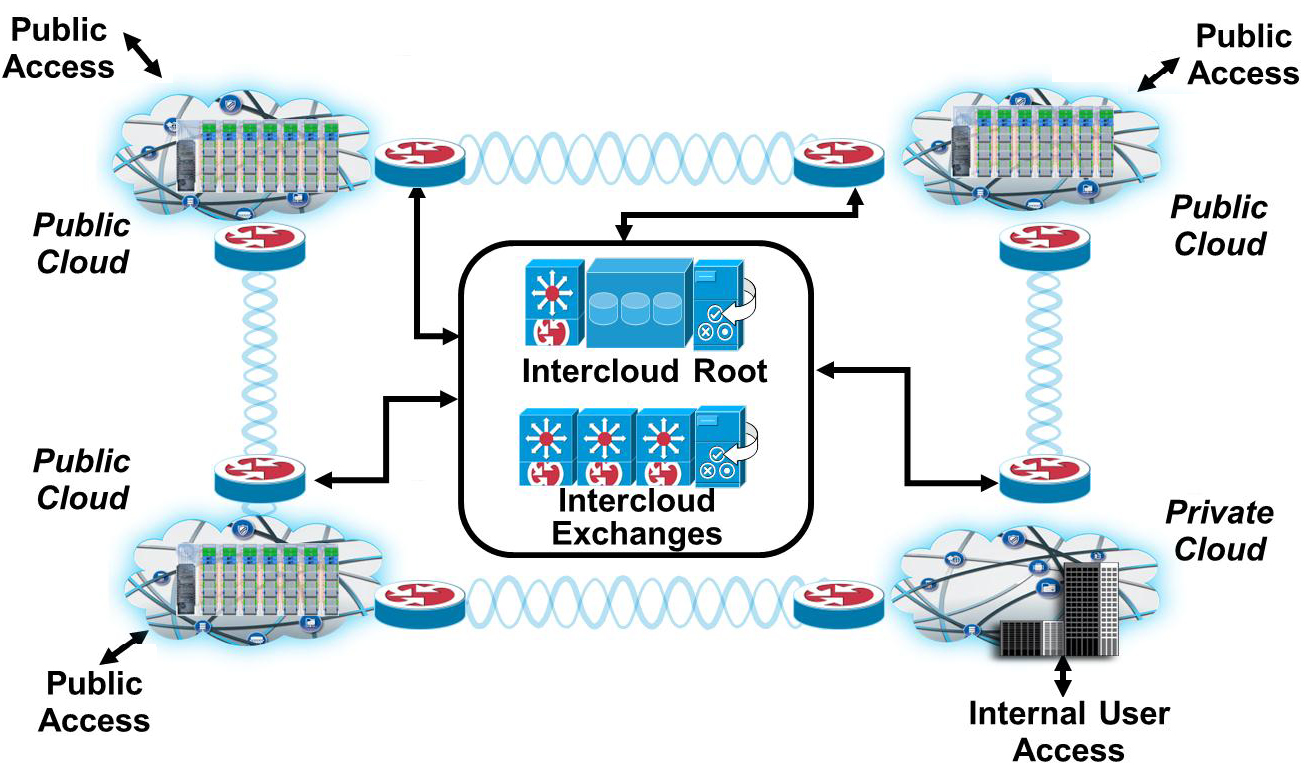
\includegraphics[width=0.7\textwidth]{img/testbed-technology.jpg}
    \caption{IEEE Intercloud Testbed Architecture}
    \label{fig:IEEE Intercloud Testbed Architecture}
\end{figure}

\subsubsection{pkgcloud}\label{par:pkgcloud}

An open source standard library that abstracts differences between several cloud providers, by offering a unified vocabulary for services like storage, compute, DNS, load balancers, so the application developer does not have to be concerned with creating different implementations for each cloud. Instead, just make the provision in the one that is most cost-effective. Currently, it only supports applications built using Node.js.

\subsubsection{Eucalyptus}\label{par:Eucalyptus}

A free and open source software to build Amazon Web Services Cloud like architectures for a private and/or hybrid Clouds. From the three solutions described, Eucalyptus is the one that is more deeply entangled with the concept of a normal Cloud, packing a: Client-side API, a Cloud Controller, S3 storage compliant modules, a cluster controller and a node controller, as seen in Figure~\ref{fig:eucalyptus}. Eucalyptus has all the components to build an entire cloud, however, since it is compatible, specially, with Amazon Cloud, we can use Eucalyptus to migrate our services, or provision Amazon services, and work without having to deal with the application or the system itself.

\begin{figure}[h!]
  \centering
  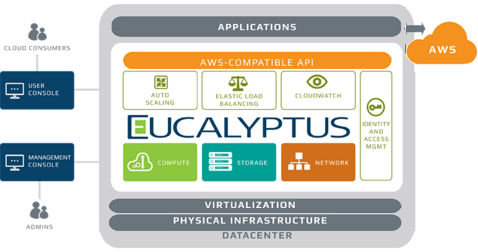
\includegraphics[width=0.7\textwidth]{img/eucalyptus-architecture.png}
  \caption{Eucalyptus Architecture}
  \label{fig:eucalyptus}
\end{figure}

This hybrid model provides a desired environment for a development, test and deploy stack, that can support Amazon Cloud with the elasticity necessary to sustain service during spikes. This way, a company that has a private cloud does not need to over provision in advance.

% 
%---------{Volunteered resource sharing}--------------------------
% 
\section{Volunteered resource sharing}

Volunteered resource sharing networks enable the cooperation between individuals to solve higher degree computational problems, by sharing idle resources that otherwise would be wasted. These individuals may or may not have a direct interest with the problem that someone is trying to solve, however they share the resources for a common good. 

The type of computations performed in this Application-level networks (ALN), are possible thanks to the definition of the problem in meta-heuristics, describing it with as laws of nature\cite{Duda2013}, such as: Evolutionary algorithms (EA); Simulated annealing (SA); Colony optimization (ACO); Particle swarm optimization (PSO), Artificial Bee Colonies (ABC) and more. This process creates small individual sets of units of computation, known as `bag of tasks', easy to distribute through several machines in and executed in parallel.
                  
% Models for distributed computation:
% Global parallelization model - One population sharded in small sets computed by several slaves
% Island Model - The population is divided in subpopulation that can run in heterogeneous machines (this is the most common in distributed computing)
% Master-Salve Model - One central pop that communicates and collects data from others              

\subsection{Hybrid and Community Clouds}

A community cloud is a network of large scale, self-organized and essentially decentralized computing and storage resources. The main focus is on free economic and censorship wise, putting the user back in control of the information, giving them freedom to share content without censorship or a company interest. The term `User Centric Cloud' appears on \cite{Barraca2011}, where the resources are made available by individuals, but with a common API, similar to a centralized Cloud, where users that participate in the effort can also use others resources.

One major trend in Community Cloud computing is not only to share and trade computing resources, but also to build the actual physical network in which they are shared, this is known as Community Networks or ``bottom-up networking''. Community Networks such as guifi.net and Athens Wireless Metropolitan Network (AWMN) have together more than 22500 nodes providing localized free access to content, without the need to contract from an Internet provider.

CONFINE\cite{Navarro} is an European effort that has the goal to federate existing community networks, creating an experimental testbed for research on community owned local IP networks. From this project, resulted Community-Lab,\footnote{http://community-lab.org/ - seen on December 2013} a federation between guifi.net, AWMN and FunkFeuer (community network from Vienna and Graz, Austria), with the goal of carrying out experimentally-driven research on community-owned open networks.


% ``Scalable, self-organized and decentralized IP networks and services built and operated by citizens for citizens'' Navarro

\subsection{Cycle and Storage Sharing, using Volunteer Resource Systems}

When we talk about peer-to-peer applications, most people will remember volunteered storage sharing, as it most widely known for its ability to distribute content, thanks to the illegal distribution of copyrighted software and media. However if we take a look at the whole spectrum of volunteer resource systems, we will see that are two categories, one for content sharing and the second one for cycle sharing, the second is known today as Public Computing.

Storage and content sharing systems are the popular type from the two categories of peer-to-peer systems, specially because their ability to distribute content without legal control, which after their success, systems like Napster\footnote{http://napster.com - seen on December 2013} were legally forced to shutdown. One of the key benefits of using a peer-to-peer storage sharing system is their ability to optimize the usage of each individual user limited bandwidth, enabling file partitioned transfers from multiple users, using the hash of each partition or chunk to prove its integrity. Each file availability grows organically with the interested in that file, because more copies will exist in the network. Other examples of this type of system are: KaZaA\footnote{http://www.kazaa.com/}, BitTorrent\footnote{http://www.bittorrent.com/} and Freenet\cite{Clarke2001}.

The second category is that of systems that fit into the domain of Public Computing, where users share their idle computer cycles; this can be done by starting or resuming a computing process when the user is not performing any task that is relevant for him/her, or by establishing the tasks as low priority processes, so it does not affect the user experience. One way of doing this is using a screen saver, so the shift to an idle state is obvious to the machine. These systems are possible because we can divide bigger computational jobs into smaller tasks that can run independently and in parallel, again this is known as the ``bag-of-tasks'' model of distributed computing. Several systems using this currently are Folding@Home, Genome@Home\cite{Larson2002} and SETI@Home\cite{Anderson2002}\cite{Korpela2001}, all BOINC\cite{Anderson2015} based. However these systems work in a one way direction: volunteers to the network do not have the possibility to use the network for its own use; nuBOINC\cite{Silva2008}, enables contributers to take advantage of the network by adding extensions to the platform that enable every user to submit jobs, adding more flexibility towards the goal in which the shared computer cycles are used. 

Another interesting research on this field is moving the logic necessary for processing some data, alongside the data, this is known as Gridlet\cite{Costa2012}\cite{Rodrigues}, a unit of workload. This approach enables a more dynamic use of volunteer resource systems with the possibility of: having different goals for the same Grid, optimize the resources available of one machine by gathering different type of tasks in one machine, reduce the cost to start using a Grid for distributed computation.

\subsection{Peer-to-Peer Networks and Architectures}  
Efficient resource discovery mechanisms are fundamental for a distributed system success, such as grid computing, cycle sharing or web application's infrastructures\cite{Ranjan2006}, although in the centralized model, by keeping data bounded inside a data center, we have a stable and scalable way for resource discovery, this does not happen in a P2P network, where peers churn rate can vary greatly, there is no way to start new machines on demand for high periods of activity, the machines present are heterogeneous and so is their Internet connectivity, creating an unstable and unreliable environment. To overcome these challenges, several researches have been made to optimize how data is organized across all the nodes, improving the performance, stability and the availability of resources. The following paragraphs will describe the current state of the art P2P organizations, typically categorized in P2P literature as Unstructured or Structured\cite{Milojicic2003}, illustrated in Figure~\ref{fig:Different types of P2P Overlay networks organizations}.

\begin{figure}[h!]
  \begin{center}
    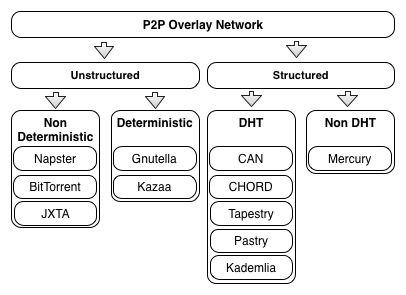
\includegraphics[width=0.70\textwidth]{./img/p2porganizations.jpg}
  \end{center}
  \caption{Different types of P2P Overlay networks organizations}
  \label{fig:Different types of P2P Overlay networks organizations}
\end{figure}


\subsubsection{Unstructured}\label{par:Unstructured}

We call `Unstructured' to a P2P system that doesn't require or define any constraint for the placement of data, these include Napster, Kazaa and Gnutella, famous for its file sharing capabilities, where nodes can share their local files directly, without storing the file in any specific Node. There is however a `caveat' in the Unstructured networks, by not having an inherent way of indexing the data present in the network, performing a lookup results of the cost of asking several nodes the whereabouts of a specific file or chunk of the file, creating a huge performance impact with an increasing number of nodes. 

In order to calibrate the performance, Unstructured P2P networks offer several degrees of decentralization, one example is the evolution from Gnutella 0.4\cite{Definition2003} to Gnutella 0.6 \cite{T.Klingberg2002}\cite{Ripeanu2002a}, which added the concept of super nodes, entities responsible for storing the lookup tables for the files in parts of the network they are responsible for, increasing the performance, but adding centralized, single points of failure. 

Unstructured networks are classified\cite{Ranjan2006} in two types: deterministic and non-deterministic, defining that in a deterministic system, we can calculate before hand the number of hops needed to perform a lookup, knowing the predefined bounds, this includes systems such as Napster and BitTorrent\cite{Cohen2009}, in which the file transfers are decentralized, the object lookup remains centralized, keeping the data for the lookup tables stored in one place, which can be gathered by one of two ways: (i) peers inform directly the index server the files they have; or (ii) the index server performs a crawling in the network, just like a common web search engine, this gives this network a complexity of O(1) to perform a search, however systems like Gnutella 0.6, which added the super node concept, remain non deterministic because it's required to execute a query flood across all the super nodes to perform the search.

\subsubsection{Structured with Distributed Hash Tables}\label{par:Structured with Distributed Hash Tables}

Structured P2P networks have an implicit way of allocating nodes for files and replicas storage, without the need of having any specie of centralized system for indexing, this is done by taking the properties of a cryptographic hash function \cite{Bakhtiari}\cite{Kargerl}\cite{Preneel1999}, such as SHA-1\cite{D.Eastlake3rdMotorola;P.JonesSystems2001}, which applies a transformation to any set of data with a uniform distribution of possibilities, creating an index with O(log(n)) peers, where the hash of the file represents the key and gives a reference to the position of the file in the network.

DHT's such as Chord\cite{Stoica2001}, Pastry\cite{Rowstron2001} and Tapestry\cite{Zhao2001}, use a similar strategy, mapping the nodes present in the network inside an hash ring, where each node becomes responsible for a segment of the hash ring, leveraging the responsibility to forward messages across the ring to its `fingers'(nodes that it knows the whereabouts). Kademlia\cite{Maymounkov} organizes its nodes in a balanced binary tree, using XOR as a metric to perform the searches, while CAN\cite{Handley} introduced and a several dimension indexing system, in which a new node joining the network, will split the space with another node that has the most to leverage.

Evaluating the DHT Structured P2P networks raises identifiable issues, that result as the trade-off of not having an centralized infrastructure, responsible for railing new nodes or storing the meta-data, these are: (i) generation of unique node-ids is not easy achievable, we need always to verify that the node-id generated does not exist, in order to avoid collisions; (ii) the routing table is partitioned across the nodes, increasing the lookup time as it scales.

Table \ref{table:p2pdht}, showcases a comparison of the studied DHT algorithms.


\begin{table}[h!]
    \begin{center}

        \begin{tabular}{| p{1.3cm} | p{2.0cm} | p{2.9cm} | p{3.2cm} | p{1.6cm} | p{1.8cm} | p{1.8cm} |}
        \hline
        \bf{P2P Algorithym} & 
        \bf{Overlay Structure} & 
        \bf{Lookup Protocol} & 
        \bf{Networking parameter} & 
        \bf{Routing table size} & 
        \bf{Routing complexity} & 
        \bf{Join/leave overhead} \\ \hline

        Chord & 
        1 dimension, hash ring & 
        Matching key and NodeID & 
        n=number of nodes in the network & 
        O(log(n)) & 
        O(log(n)) & 
        O(log(n)\textsuperscript{2}) \\ \hline

        Pastry & 
        Plaxton style mesh structure & 
        Matching key and prefix in NodeID & 
        n= number of nodes in the network, b=base of identifier & 
        O(log\textsubscript{b}(n) & 
        O(b log\textsubscript{b}(n) + b) & 
        g \\ \hline

        CAN & 
        d-dimensional ID Space & 
        Key value pair map to a point P in D-dimensional space & 
        n=number of nodes in the network, d=number of dimensions & 
        0(2d) & 
        O(d n\textsuperscript{1/2}) & 
        O(2d) \\ \hline

        Tapestry & 
        Plaxton style mesh structure & 
        Matching suffix in NodeID & 
        n=number of nodes in the network, b=base of the identifier & 
        O(log\textsubscript{b}(n)) & 
        O(b log\textsubscript{b} (n)+b) & 
        O(log(n)) \\ \hline

        Kademlia & 
        Binary tree & 
        XOR metric & 
        n=number of nodes, m=number of bits(prefix) & 
        O(log(n)) & 
        O(log\textsubscript{2}(n)) & 
        not stable \\ \hline

        \end{tabular}
    \end{center}
\caption{Summary of complexity of structured P2P systems}
\label{table:p2pdht}
\end{table}	


\subsubsection{Structured without Distributed Hash Tables}\label{par:Structured without Non-Distributed Hash Tables}

Mercury\cite{Bharambe}, a structured P2P network that uses a non DHT model, was designed to enable range queries over several attributes that data can be dimensioned on, which is desired on searches over keywords in several documents of text. Mercury design offers an explicit load balancing without the use of cryptographic hash functions, organizing the data in a circular way, named `attribute hubs'.

\subsubsection{Fault Tolerance, Load Balancing, Assurance and Trust}

Volunteer resource sharing means that we no longer have our computational infrastructure confined in a well monitored place, introducing new challenges that we have to address \cite{Koloniari2005} to maintain the system running with the minimum service quality. These issues can be: scalability, fault tolerance, persistence, availability and security\cite{Wallach} of the data and that the system doesn't get compromised. This part of the document serves to describe the techniques implemented in previous non centralized systems to address this issues.

\subsubsection{Fault Tolerance, Persistence and Availability}\label{par:Fault Tolerance, Persistence and Availability}

are one of the key challenges in P2P community networks, due to it's churn uncertainty, making the system unable to assume the availability of Node storing a certain group of files. Previous P2P systems offer a Fault Tolerance and Persistence by creating file replicas, across several Nodes in the network, one example is PAST\cite{Rowstron2001}\cite{Rowstron2001a}, a system that uses PASTRY routing algorithm, to determine which nodes are responsible to store a certain file, creating several different hashes which corresponds to different Nodes, guaranteeing an even distribution of files across all the nodes in the network. DynamoDB\cite{Decandia2007}, a database created by Amazon to provided an scalable NOSQL solution, uses a storage algorithm, inspired by the Chord routing algorithm, in which stores file replicas in the consequent Nodes, in order to guarantee easy lookup if one of the Nodes goes down.

The strategy presented by the authors of PAST to provide high availability, is an intelligent Node system, that use a probabilistic model, able to verify if there is an high request for a file, deciding to keep a copy and avoiding to overload the standard Node with every request that is made.

\subsubsection{Load Balancing}\label{par:load_balancing}

in an optimal state, can be defined as having each node sharing roughly 1/N of the total load inside the network, if a Node has a significantly hight load compared with the optimal distribution, we call it a `heavy' node. There has been some research to find a optimal way to balance the load inside a P2P network, namely:

\begin{itemize}
   \item Power of Two Choices\cite{Byers} - Uses multiple hash functions to calculate different locations for an object, opts to store it in the least loaded node, where the other Nodes store a pointer. This approach is very simple, however it adds a lot of overhead when inserting data, however there is a proposed alternative of not using the pointers, which has the trade-off of increasing the message overhead at search.
   \item Virtual Servers\cite{Rao2003} - Presents the concept of virtualizing the Node entity to easy transfer it amongst the machines present in the P2P network. It uses two approaches, `one-to-one', where nodes contact other Nodes inside the network with the expectation of being able to trade some of the load, shifting a virtual server, or an `one-to-many/many-to-many' in which a directory of load per node is built, so that a node can make a query in order to find it's perfect match to distribute his load. Virtual Servers approach has the major issue of adding a extra amount of work to maintain the finger tables in each node.
   \item Thermal-Dissipation-based Approach\cite{Rieche} - Inspired by the heat expansion process, this algorithm shifts nodes position inside the hash ring windows of load responsibility, in a way that the load will implicitly flow from a node to it's close peers.
   \item Simple Address-Space and Item Balancing\cite{Karger2004} - It is an iteration over the virtual servers, by assigning several virtual nodes to each physical node, where only one of which is active at a time and this is only changed if having a different nodeId distribution in the network brings a more load balanced hash ring
 \end{itemize} 

S. Rieche, H. Niedermayer, S. Götz and  K. Wehrle from the University of Tübingen, made a study comparing this different approaches in a scenario using the CHORD routing algorithm, using a SHA-1 as the hashing function, with 4096 nodes and 100.000 to 1.000.000 documents and executing up to 25 runs per test, the results can be observed in the Figure ~\ref{fig:lbcomp}

\begin{figure}[h!]
    \centering
    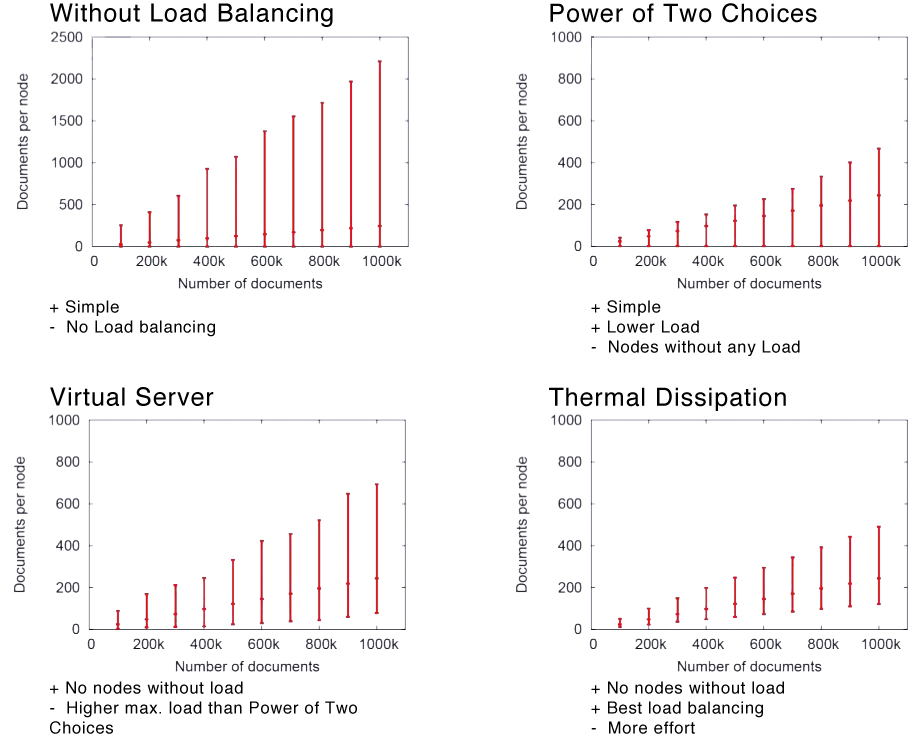
\includegraphics[width=0.7\textwidth]{img/lb.jpg}
    \caption{Load balancing approaches comparison}
    \label{fig:lbcomp}
\end{figure}

\subsubsection{Assurance and Trust}\label{par:Assurance and Trust}

in a P2P network is an interesting challenge due to the lack of control over the machines that are willing to share with their resources, in order to achieve it, several strategies have been developed to maintain the integrity of the data using Cryptography, Reputation modeling schemes based on it's node previous record and also economic models, that resemble our own economy, but to share and trade computational resources.

Starting with the Cryptographic techniques, storage systems such as PAST give the option to the user to store encrypted content, disabling any other user, that does not have the encryption key, to have access to the content itself, this is a technique that comes from the Client-Server model, adapted to P2P environment, however, other cryptography technique benefits such as user authorization and identity, cannot be directly replicated into a P2P network without having a centralized authority to issue this validations, one of the alternatives is using distributed signature strategy, known as Threshold Cryptography \cite{Desmedt;1998}, where an access is granted if validated if several peers (a threshold), validates it's access, one implementation of Threshold Cryptography can be see in a P2P social network\cite{Afify} in order to guarantee privacy over the contents inside the network. 

Trust in a P2P system, as mentioned, is fundamental to it's well behaved functioning, not only in terms of data privacy, but also in giving the deserved resources to the executions that mostly need them, avoiding misbehaved peer intentions that can be a result of an Attack to jeopardize the network, one example is the known Sybil attack\cite{Douceura}. To achieve a fair trust sharing system, several metrics for a reputation mechanism have been developed \cite{Marti}, these can be seen in Table \ref{table:reputation}.

\begin{table}
    \centering
    \begin{tabular}{| c | c | c |}
        \hline                        
        \multicolumn{3}{|c|}{Reputation Systems} \\

        \hline                        
        Information Gathering & Scoring and Ranking & Response \\

        \hline                        
        Identity Scheme & Good vs. Bad Behavior & Incentives \\
        Info. Sources & Quantity vs. Quality & Punishment \\
        Info. Aggregation & Time-dependence &   \\ 
        Stranger Policy & Selection Threshold &   \\ 
            & Peer Selection &   \\ 

        \hline                           
    \end{tabular}
    \caption{Reputation system components and metric}
    \label{table:reputation}
\end{table}

Incentives for sharing resources\cite{Golle2001} can in the form of money rewards, greater speed access(used in Napster and some bittorrent networks) or it can be converted to a interchangeable rate to trade for more access to resources, giving the birth of economic models\cite{Filipe2011}\cite{Vishnumurthy}, that model the traded resources as a currency in which a peer has to trade in order to use the network.

% Economic Models
% * Gridlet Economics: Resource Management Models and Policies for Cycle-Sharing Systems
% * KARMA : A Secure Economic Framework for Peer-to-Peer Resource Sharing  (note: stores reputation remotly) Nead to Read

% 
%---------{Resource sharing using the Web as platform}------------
% 
\section{Resource sharing using the Web platform} 

One of the main focuses with the proposed work, is to take advantage of the more recent developments of the Web platform to make the intended design viable (presented in section 4), the system depends on very lower level components such as:
\begin{itemize}
    \item High dynamic runtime for ongoing updates to the platform and specific assets for job execution
    \item Close-to-native performance for highly CPU-bound jobs
    \item Peer-to-peer interconnectivity
    \item Scalable storage and fast indexing
\end{itemize}

Therefore, we present in this section the relevant components present or undergoing a development process for the Web platform, such as: Javascript, Emscripten, IndexedDB, WebRTC and HTTP2.0. These will coexist as key enablers for  the necessary features to such a distributed shared resource system:

\subsection{Web Platform}

Since the introduction of AJAX\cite{Google/Mozzila/Opera}, the web has evolved into a new paradigm where it left being a place of static pages, known as Web 1.0. Nowadays, we can have rich web applications with degrees of interaction and levels of performance close to a native application. The programming languages that power the Web Platform, in special HTML, CSS and JavaScript\cite{Ecma2009}, have been subject to several changes, enabling `realtime' data transfers and fluid navigations through content. Javascript, an interpreted language with an high dynamic runtime, has proven to be the right candidate for a modular Web Platform, enabling applications to evolve continuously over time, by simply changing the pieces that were updated.

\textbf{Emscripten}\cite{Zakai2011}, a LLVM(Low Level Virtual Machine) to JavaScript compiler, enabled native performance on Web apps by compiling any language that can be converted to LLVM bytecode, for example C/C++, into JavaScript. This tool enabled native game speed on the browser, where two of the major examples are the project Codename: ``BananaBread''\footnote{Mozilla, BananaBread,  URL: https://developer.mozilla.org/en/demos/detail/bananabread, seen in December 2013} and ``Epic Citadel''\footnote{Mozilla, Epic Citadel,  URL: http://www.unrealengine.com/html5/, seen in December 2013}, in which Mozilla used Ecmascripten to port the entire Unreal Engine 3 to JavaScript. In Figure~\ref{fig:dan}, we can see a comparison of the performance of several algorithms, running on Dalvik, Android Java runtime, asm.js, the subset of Javascript that the code in C/C++ is transformed into when compiled with Emscripten and Native, the same C/C++ but running on a native environment. The results are very interesting, specially in the first test, where asm.js outperforms native. The explanation for this is due to the fact that BinaryTrees use a significant amount of `malloc' invocations, which is an expensive system call, where in asm.js, the code uses typed arrays, using `machine memory', which is flat allocated in the beginning of the execution for the entire run.

\begin{figure}[h!]
  \centering
  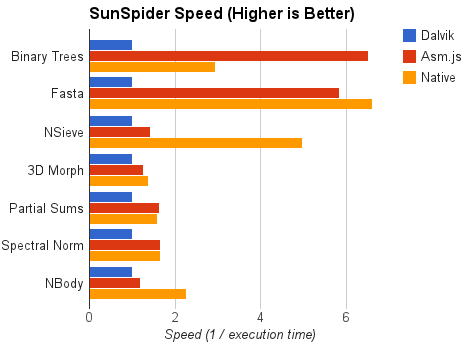
\includegraphics[width=0.65\textwidth]{img/Dalvik-vs-ASM-vs-Native-edited}
  \caption{Dalvik vs. ASM.js vs. Native performance}
  \label{fig:dan}
\end{figure}

\textbf{WebRTC}\footnote{http://www.w3.org/TR/2013/WD-webrtc-20130910/}, a technology being developed by Google, Mozilla and Opera, with the goal of enabling Real-Time Communications in the browser via a JavaScript API. WebRTC brings to the browser the possibility of peer-to-peer interoperability. Peers perform their handshake through a `Signaling Server'. The signaling server will exchange the `ICE(Interactive Connectivity Establishment) candidates' of each peer as this serves as an invite so a data-channel can be opened, a visualization of this process can be seen in Figure~\ref{fig:webrtc}. Since most of the browsers sit behind NAT, there is another server, named `Turn'(Relay), which tells to each browser their public IP in the network. WebRTC, although being built with the goal of real-time voice and video communications, has also been shown as a viable technology do distribute content, as seen in PeerCDN and SwarmCDN\cite{Vogt}.

\begin{figure}[h!]
  \centering
  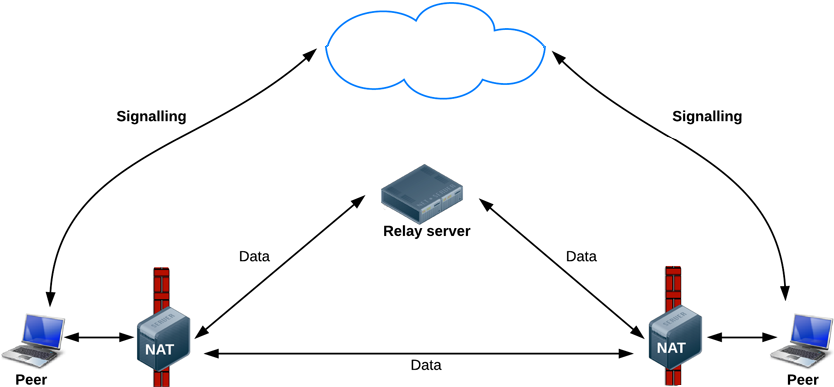
\includegraphics[width=0.65\textwidth]{img/webrtc.png}
  \caption{Example of a WebRTC session initiation}
  \label{fig:webrtc}
\end{figure}

% 
% There is also Jingle
% https://github.com/legastero/jingle.js
% Jingle is an extension of XMPP that enables P2P and communication over RTC
% 

\textbf{`level.js'} offers an efficient way to store larger amounts of data in the browser machine persistent storage, its implementation works as an abstraction on top of the leveldown API on top of IndexedDB\footnote{http://www.w3.org/TR/2014/WD-service-workers-20141118/}, which in turn is implemented on top of the LevelDB\footnote{http://www.w3.org/TR/2013/WD-webrtc-20130910/}, an open source on-disk key-value store inspired by Google BigTable. IndexedDB is an API for client-side storage of significant amounts of structured data and for high performance searches on this data using indexes. Since `level.js' runs on the browser, we have an efficient way to storage data and quickly retrieve it.

One of the latest improvements being built for the Web Platform is the new HTTP spec, \textbf{HTTP2.0}\cite{Thomson2013}, this next standard after HTTP1.1 which aims to improve performance towards a more realtime oriented web, while being retrocompatible at the same time. Several advancements in this new spec are:

\begin{itemize}
  \item Parallel requests - HTTP1.1 was limited by a max of 6 parallel requests per origin and taking into account that the mean number of assets is around one hundred when loading an webapp, it means that transfers get queued and slowed down. In order to overcome this, we could distribute the assets through several origins in order to increase the throughput. However this optimization backfired when in mobile, since there was a lot of signaling traffic in TCP layer, starving the user connection. HTTP2.0 no longer has this constraint.
  \item Diff updates - One of the web developer favorites has been concatenating their javascript files so the response payload decreases, however, in modern webapps, most of the time, we do not want the user to download the entire webapp again, but only some lines of code referring to the latest update. With diff updates, the browser will only receive what has been changed.
  \item Prioritization and flow control - Different webapp assets have different weights in terms of user experience, with HTTP2.0, the developer can set priorities so the assets arrive by order.  A simple flow control example can be seen on Figure~\ref{fig:http2dataflow}, where the headers of the file gain priority as soon as they are ready, and get transfered immediately. 
  \item Binary framing - In HTTP2.0, binary framing is introduced with the goal of creating more performant HTTP parsers and encapsulating different frames as seen on Figure~\ref{fig:binaryframing}, so they can be send in an independent way.
  \item HTTP headers compression - HTTP2.0 introduces an optimization with headers compression\cite{Ruellan2013} that can go to a minimum of 8 bytes in identical requests, against the 800 bytes in HTTP1.1. This is possible because of the state of the connection is maintained, so if a identical requests is made, changing just one of the resources (for example path:/user/a to path:/user/b), the client only has to send that change in the request.
  \item Retrocompatibility - HTTP2.0 respects the common headers defined by HTTP1.1, it doesn't include any change in the semantics.
\end{itemize}

\begin{figure}[h!]
  \centering
  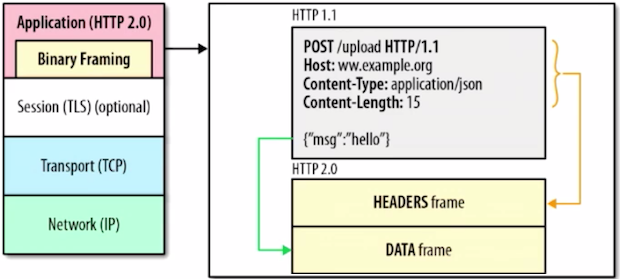
\includegraphics[width=0.65\textwidth]{img/http2binaryframing.png}
  \caption{HTTP2.0 Binary framing}
  \label{fig:binaryframing}
\end{figure}

\begin{figure}[h!]
  \centering
  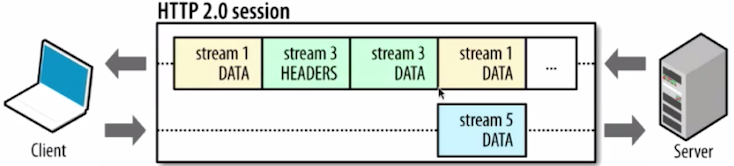
\includegraphics[width=0.65\textwidth]{img/http2dataflow.png}
  \caption{Example of an HTTP2.0 dataflow}
  \label{fig:http2dataflow}
\end{figure}

\subsection{Previous attempts on cycle sharing through web platform}
The first research of browser-based distributed cycle sharing was performed by Juan-J. Merelo, et. al., which introduced a Distributed Computation on Ruby on Rails framework\cite{Merelo2007}. The system used a client-server architecture in which clients, using a browser would connect to a endpoint, where they would download the jobs to be executed and sent back the results. In order to increase the performance of this system, a new system\cite{Duda2013} of browser-based distributed cycle sharing was creating using Node.js as a backend for very intensive Input/Output operations\cite{Tilkov2010}, with the goal of increased efficiency, this new system uses normal webpages (blogs, news sites, social networks) to host the client code that will connect with the backend in order to retrieve and execute the jobs, while the user is using the webpage, this concept is known as parasitic computing\cite{Barabasi2001}, where the user gets to contribute with his resources without having to know exactly how, however since it is Javascript code running on the client, any user has access to what is being processed and evaluate if it presents any risk to the machine.

\section{Summary}

The related work presented was researched with the goal of deepen the knowledge about current strategies for resource sharing, as we intend to present a new one using the Web Platform. The concept of Gridlet, akin to those seen as well in state of the art databases such as Joyent's Manta,\footnote{http://www.joyent.com/products/manta - seen in December 2013} which bring the computation to/with the data, reducing the possibility of a network bottleneck and increases the flexibility to use the platform for new type of jobs, will very important. To enable this new Cloud platform on using browsers, it is important to understand how to elastically scale storage and job execution, as in \cite{Silva2011}, but in peer-to-peer networks: therefore a study of the current algorithms and its capabilities was needed. Lastly, browsing the web has been around for almost 20 years, hower on the last few, we are seeing the Web Platform rapidly changing, and enabling new possibilities with peer-to-peer technology e.g. WebRTC; otherwise, it would not be possible to create browserCloud.js.

    %%!TEX root = ../document.tex
\chapter{Architecture}\label{ch:architecture}

\begin{quotation}
    “The possibility of that which has never occurred cannot be determined by opinion—only by an attempt.”
    {\small\it -- Dee Hock Biography, One From Many}
\end{quotation}

browserCloud.js proposes a mechanism to find, gather and utilize idle resources present in a P2P overlay network, in which its participants will be joining and connecting to each other through a rendezvous point, as represented in Figure~\ref{fig:b-e}. For a given peer, all that the peer needs to know is that once part of this network, it can submit a job which will be partitioned and distributed across a number of peers available, being responsible for later aggregating the results and delivering them to the user which summoned that job. The user does not need to understand how the network is organized or which peers it is directly connected too, so that complexity is abstracted by browserCloud.js.

\begin{figure}[h!]
  \centering
  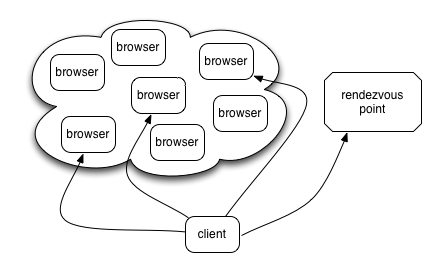
\includegraphics[width=0.7\textwidth]{figs/birds-eye}
  \caption{browserCloud.js Overview}
  \label{fig:b-e}
\end{figure}

A pratical use case for browserCloud.js is high CPU bound jobs and capable to run in parallel, e.g: image processing, video compressing, data manipulation, map and reduce functions, etc. These parallel tasks are divided by the peers available in the network, leveraging the parallelism to obtain a speed up.

This chapter describes the architecture designed for the browserCloud.js system. browserCloud.js was designed with with the Unix philosophy, that is, subtracting the unnecessary from a subsystem until it is constructed to perform one thing and one thing well, building more cohese abstractions through composition.

browserCloud.js was architectured to meet the following requirements:

\begin{itemize}
    \item \textbf{Membership management} - The system has to enable peers to join and leave a current network of browserCloud.js peers or a subset of it. A peer should only have the knowledge of a small of other peers in the network and be available to rail in any other peer that wants to be part of the P2P network.
    \item \textbf{Message routing} - Peers must have a way to communicate with every other peer in the network without the necessity of contacting a centralized service to do so. Messages should be routed between peers, having each peer knowing a subset of the network, guaranteeing in full coverage in this manner.
    \item \textbf{Job scheduling and results aggregation} - The discovery of computational resources must be performed using a distributed approach, peers interact between each other to send tasks and retrieve the results for the peer executing the job.
    \item \textbf{Support dynamic runtime} - Provide flexibility for jobs being executed. This is delivered thanks to the dynamic runtime offered by by peers in browserCloud.js due to the fact that they are standard compliant web browsers and Javascript is the language used.
    \item \textbf{Reduced entrance cost to enable greater adoption} - Designed simple APIs, abstracting the complexity in favor of greater extendability.
\end{itemize}

\section{Distributed Architecture}

The overview of the distributed architecture can be seen in Figure~\ref{fig:n-a-o}.

\begin{figure}[h!]
  \centering
  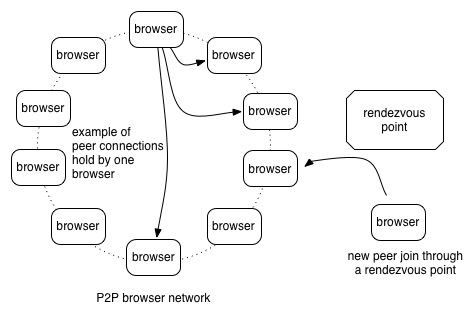
\includegraphics[width=0.7\textwidth]{figs/network-architecture-overview}
  \caption{browserCloud.js Distributed Architecture Overview}
  \label{fig:n-a-o}
\end{figure}

\subsection{Entities}

There are two different kind of actors in the system:

\begin{itemize}
    \item browser - The points on our network that will be able to issue jobs, execute tasks and route messages.
    \item rendezvous point - The only centralized component in this architecture, its purpose is for the clients to have a way to connect to and join the overlay network. 
\end{itemize}

\subsection{Interaction Protocols}

In a browserCloud.js infrastructure, we have three main interaction patterns, the first being when a peer joins or leaves the network, which also we can call membership management, something that in traditionally P2P networks would simply mean an exchange of a IP:Port pair, but in a P2P browser network, a RTCPeerConnection has to be established and kept alive, meaning that an handshaking protocol must be performed. The second pattern is message routing between peers, this has been designed with inspiration on the Chord\cite{Stoica2001},routing algorithm, studied on the related work. The third interaction demonstrates how to levarage the computer cycles available in the network to process CPU bound jobs.

\subsubsection{Peer joins and leaves}

A peer join compromisses of the following steps:

\begin{itemize}
    \item \textbf{1 - Registration} - When a peer is ready to join the network, it performs the registration action to the custom browserCloud.js signalling server, the server replies with a confirmation and a unique ID for this peer to occupy in the network. This enables the signalling server, which holds the meta data of the current state in the network, to pick the ID in the ID interval that might be less occupied. We can observe this interaction in Figure~\ref{fig:1-p-r}.
    \item \textbf{2 - New peer available} - As peers join the network, other peers present need to be notified to establish or update their connections to the new best candidates, so that the routing of messages (explained in the next section), remains efficient. For each peer join, a notification with a finger update can be sent to 1 or more peers present, as seen in Figure~\ref{fig:2-p-n}.
    \item \textbf{3 - Connection establishment between two peers} - In order to establish a connection between two peers, once there is an interest for these to connect, for e.g, in the case of a finger update event. There are two substeps, the first being the SDP offer creation through a technique called "hole punching", where a browser uses one of the WebRTC API to traverse through NAT to obtain its public IP, which is crucial information when two browsers need to establish a direction connection, Figure~\ref{fig:3-p-s}. The second step is the exchange of these SDP offers between browsers and that has to be performed by a centralized service; in browserCloud.js we developed a custom signalling server that handles that part, as seen in Figure~\ref{fig:4-p-c}.
\end{itemize}

A peer leave is a simpler and organic process, once a peer leaves the network, the RTCPeerConnections objects are closed and destroyed, notifying automatically the peers that have to update their finger tables that they should request the signalling server to update the metadata of the state of the network and therefore, issuing new finger-update messages.

The meta state of the network is always held in memory by the signalling server, there is no need to keep this state persistent because it can be easily reconstructed, in the event of the signalling server failing, a new instance can be spawn and the peers simply have to register again, but this time with their current IDs.

\begin{figure}[h!]
  \centering
  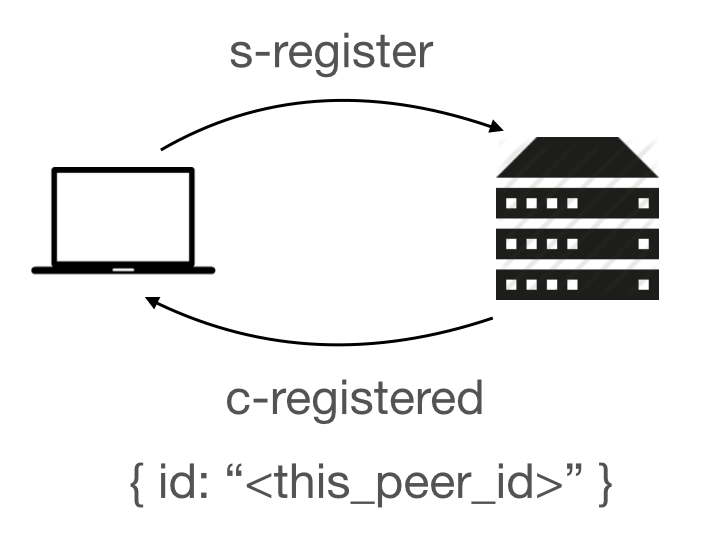
\includegraphics[width=0.4\textwidth]{figs/1-peer-registers}
  \caption{Registration of a peer, signaling itself as available to be part of the P2P network}
  \label{fig:1-p-r}
\end{figure}

\begin{figure}[h!]
  \centering
  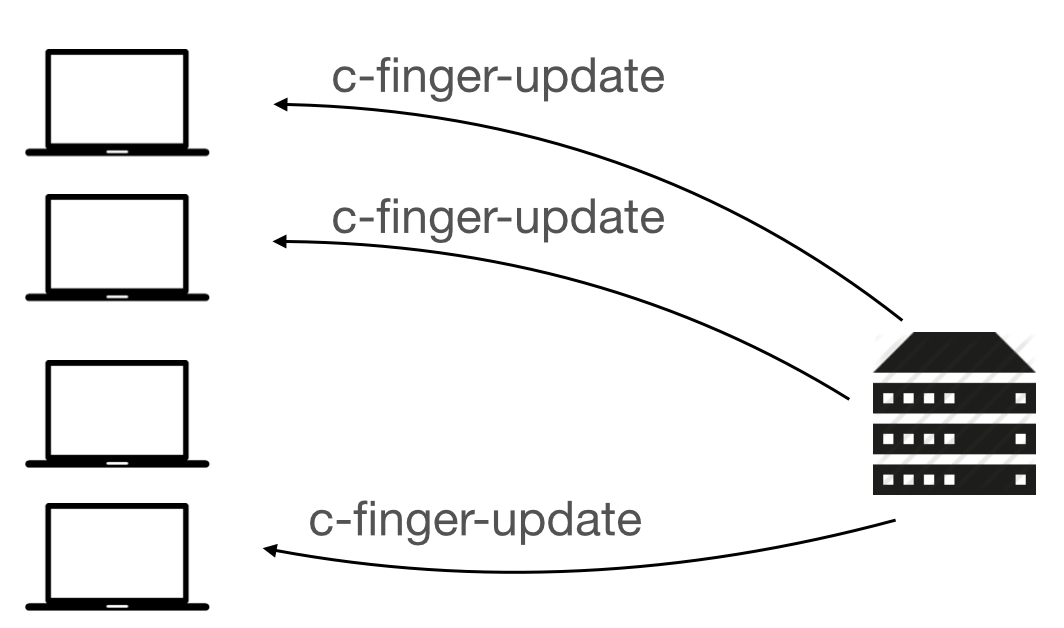
\includegraphics[width=0.4\textwidth]{figs/2-peers-notified}
  \caption{A peer is notified to update his finger table}
  \label{fig:2-p-n}
\end{figure}

\begin{figure}[h!]
  \centering
  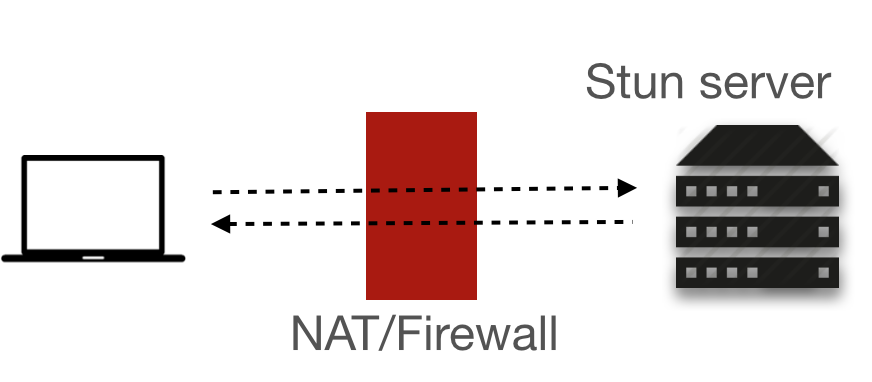
\includegraphics[width=0.4\textwidth]{figs/3-peer-stun}
  \caption{Hole punching through NAT to obtain a public IP and create a SDP offer}
  \label{fig:3-p-s}
\end{figure}

\begin{figure}[h!]
  \centering
  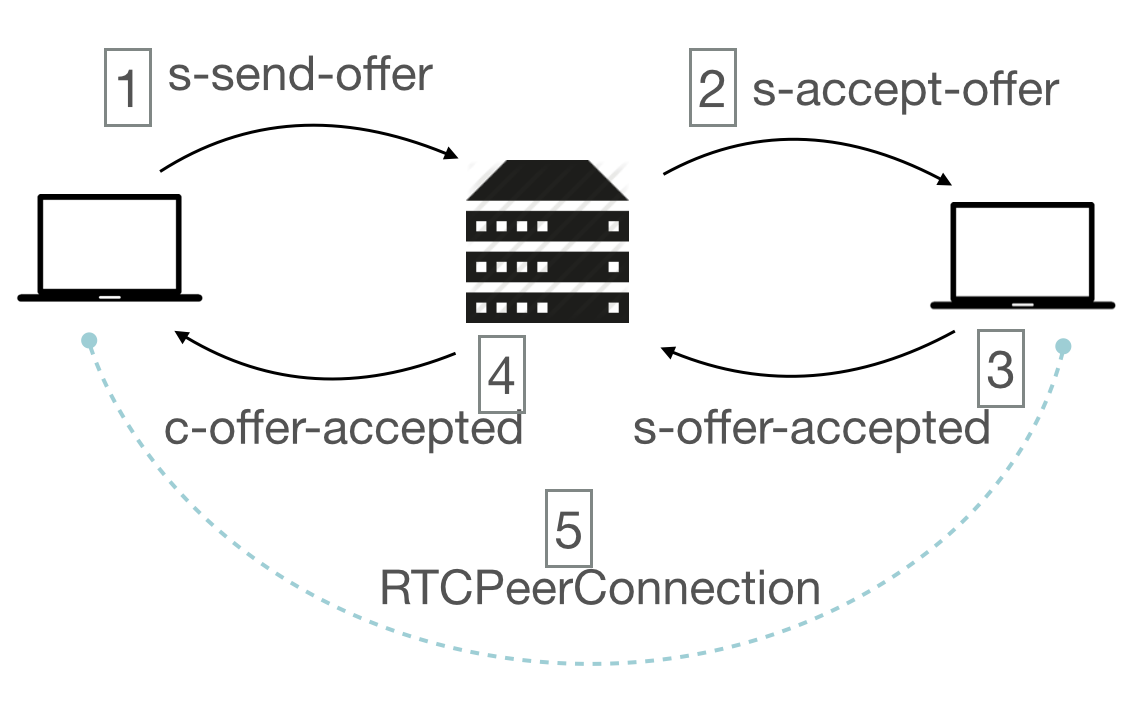
\includegraphics[width=0.4\textwidth]{figs/4-peer-connect}
  \caption{Establishment of a RTCPeerConnection through the custom Signalling Server}
  \label{fig:4-p-c}
\end{figure}

\subsubsection{Message routing}

For message routing, we designed an adaptation of the Chord routing algorithm, a P2P Structured Overlay network, a DHT studied in the related work, with the goal of keeping an efficient routing and resource lookup with the increase of the number of peers in the network.

The ID namespace available in our DHT consists of 48 bit IDs (Figure~\ref{fig:c-1} ), this decision was made due to the fact that Javascript only supports 53 bit numbers, to support a greater variaty of IDs, we would have to resort to a big integer third party library, adding unnecessary consuption of computing resources. However, for demonstration purposes, we will explain using a 3 bit ID namespace.

\begin{figure}[h!]
  \centering
  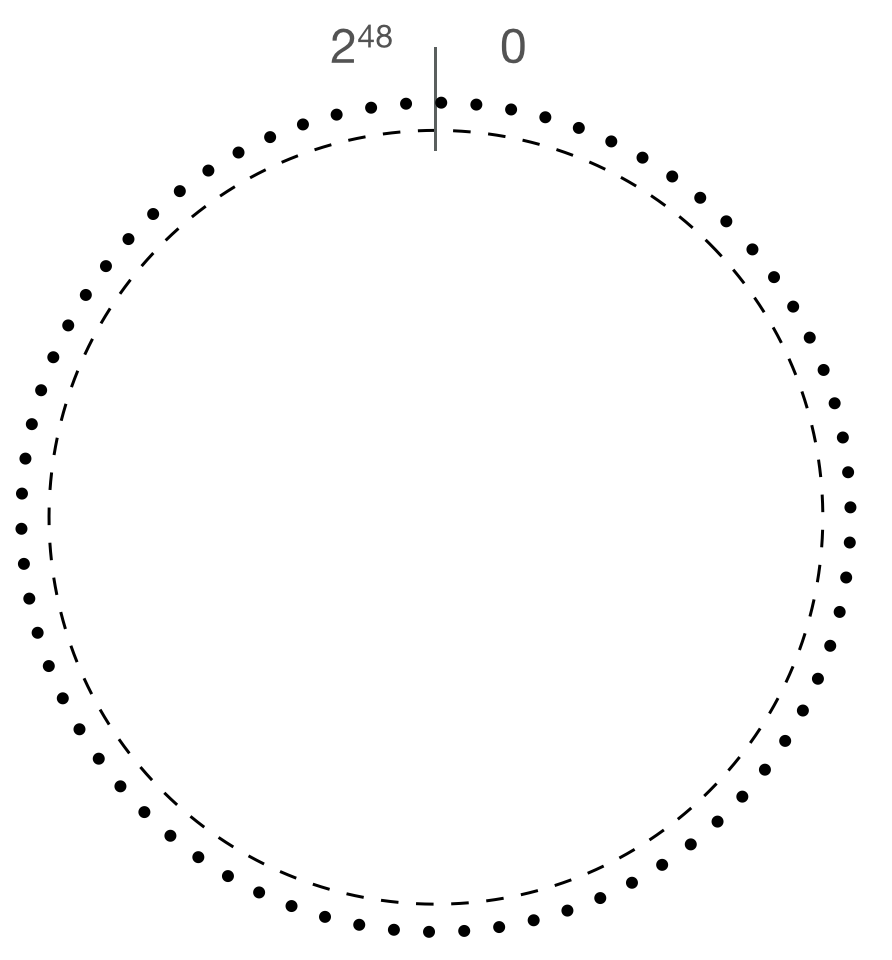
\includegraphics[width=0.4\textwidth]{figs/chord-1}
  \caption{How the ID namespace is visualized in the DHT}
  \label{fig:c-1}
\end{figure}

In Figure~\ref{fig:c-2}, we have a DHT composed of 4 different peers, with IDs 0, 1, 3 and 6. Each one of these peers will be responsible for a segment of the DHT, in another words what this means is that every message that is destined to their segment, will be delivered to respective peer responsable. A peer is responsible for a segment of IDs greater than the peer that is its predecessor and lesser or equal than its own ID, represented in Figure ~\ref{fig:c-3}. When a peer enters in the network, its ID is generated through a crop of a SHA-1 hash from a random generated number, creating a natural uniform distribution.

\begin{figure}[h!]
  \centering
  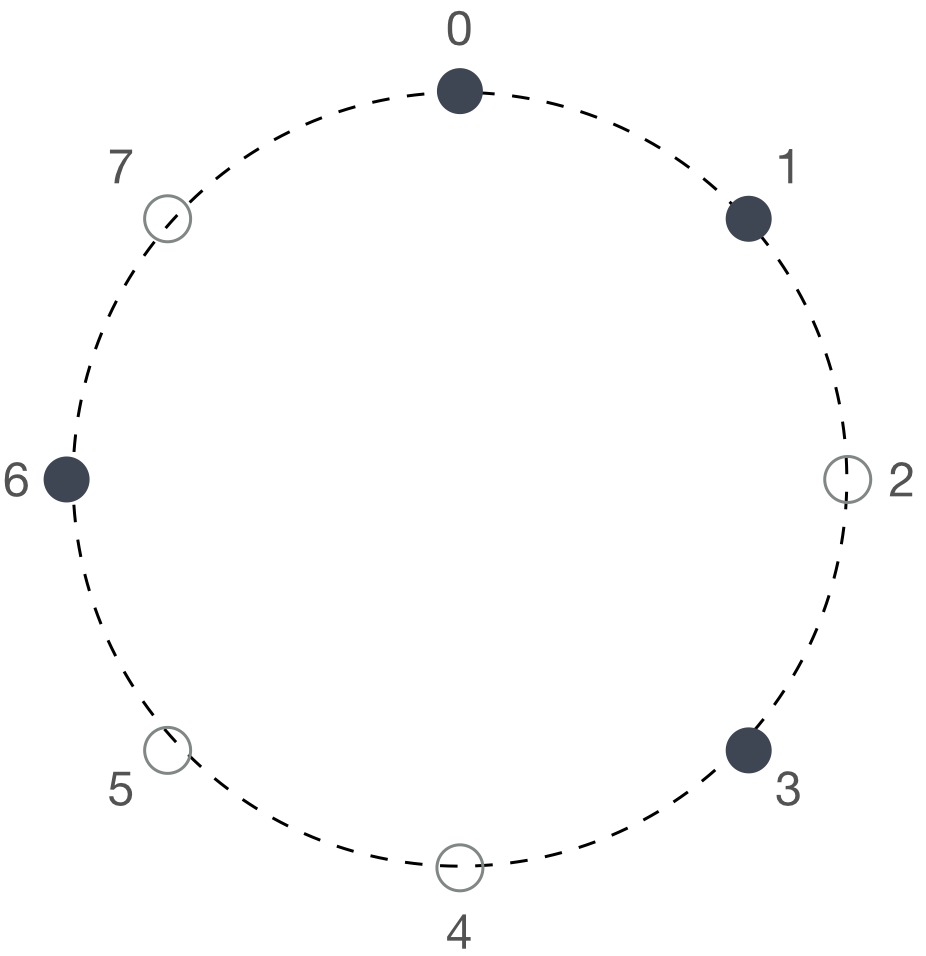
\includegraphics[width=0.4\textwidth]{figs/chord-2}
  \caption{Example of a DHT with 4 peers for case study}
  \label{fig:c-2}
\end{figure}

\begin{figure}[h!]
  \centering
  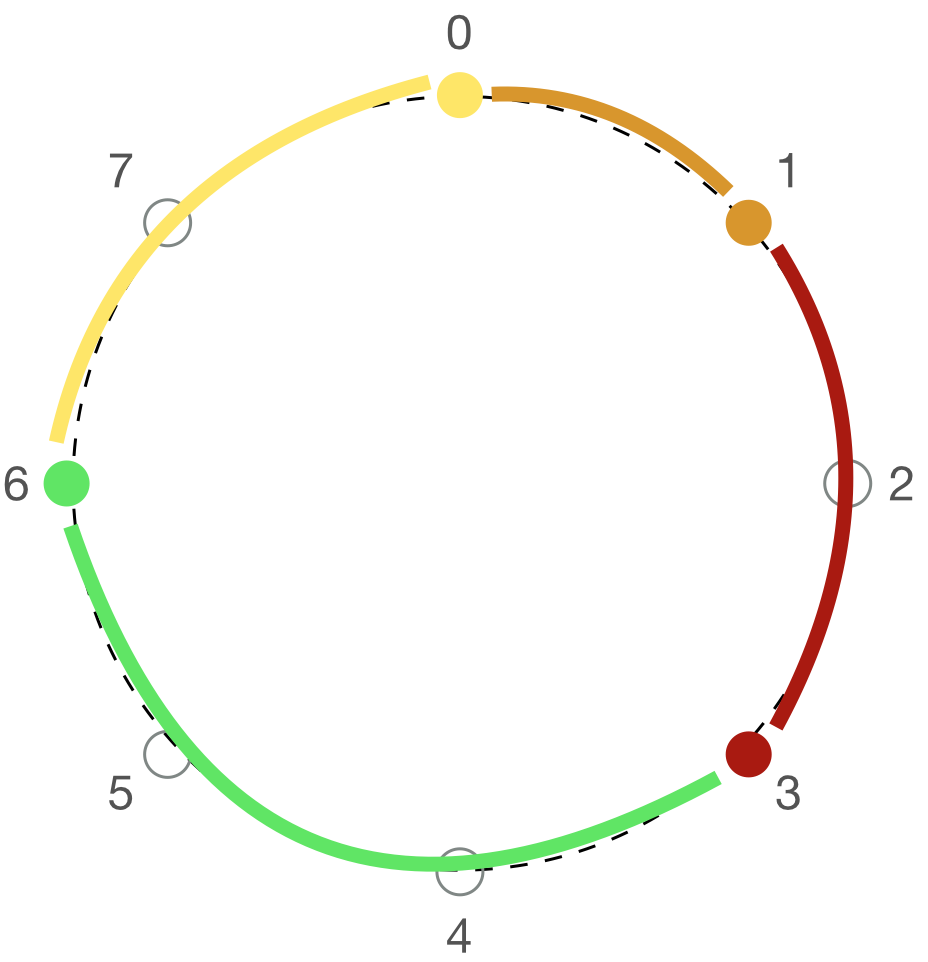
\includegraphics[width=0.4\textwidth]{figs/chord-3}
  \caption{Responsability interval for each Peer}
  \label{fig:c-3}
\end{figure}

In order for messages to find its correct destination, each peer has to know at minimum the peer that is next to it on the DHT, also called "successor" (Figure~\ref{fig:c-4}). Messages will be forward until they reach the peer which compromisses the responsability of being responsible for that message ID.

\begin{figure}[h!]
  \centering
  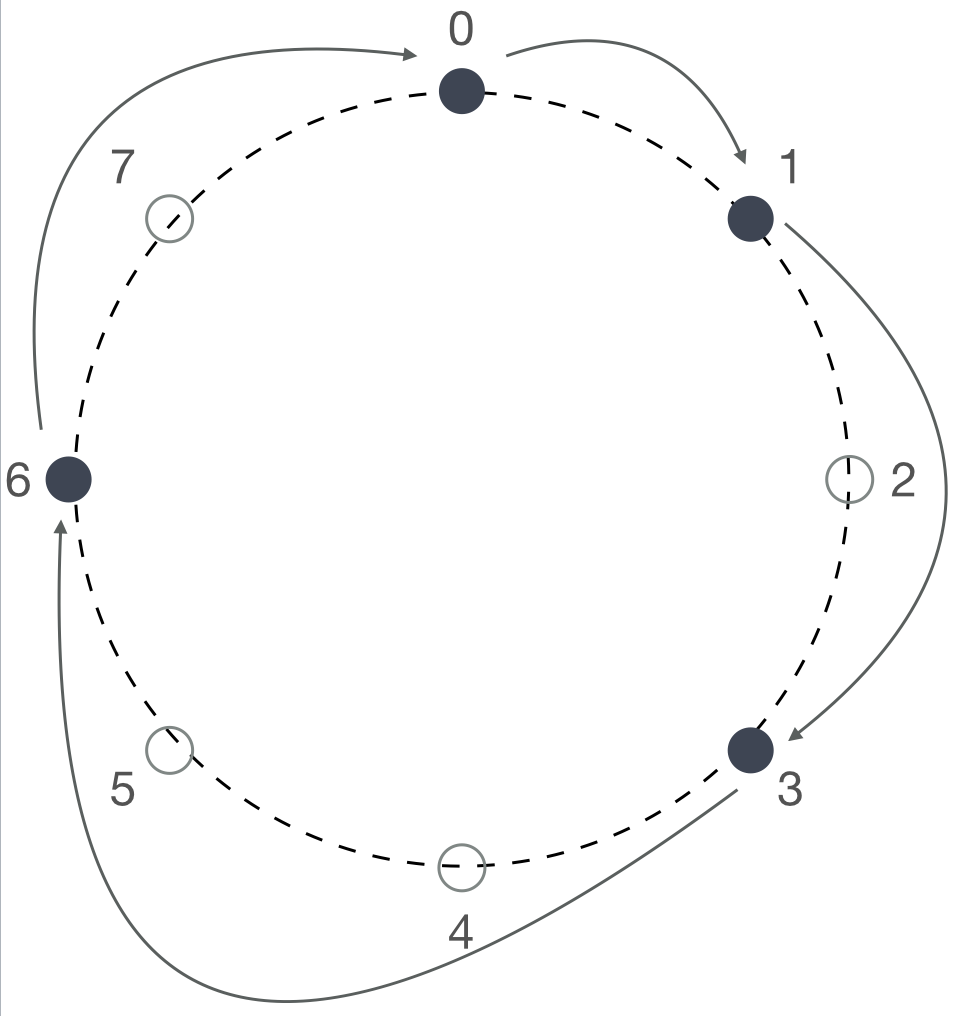
\includegraphics[width=0.4\textwidth]{figs/chord-4}
  \caption{Minimum number of connections for messages to be routed properly}
  \label{fig:c-4}
\end{figure}

However, as specified earlier in the document, we want to achieve a good and stable efficiency when it comes to routing messages inside the DHT as the network grows. To achieve that, we introduce fingers in our peers as we mentioned earlier. A finger is a direct connection to another peer in the network (Figure~\ref{fig:c-5}), that was picked following a specific distribution, each peer will have 1 to N fingers, where N is the number of bits of the IDs (for this example, N = 3). A finger is always the peer responsible for the "start" value of the interval (see Figure~\ref{fig:c-6} for reference and formula) and a message will be routed to that finger if it falls inside the interval.

\begin{figure}[h!]
  \centering
  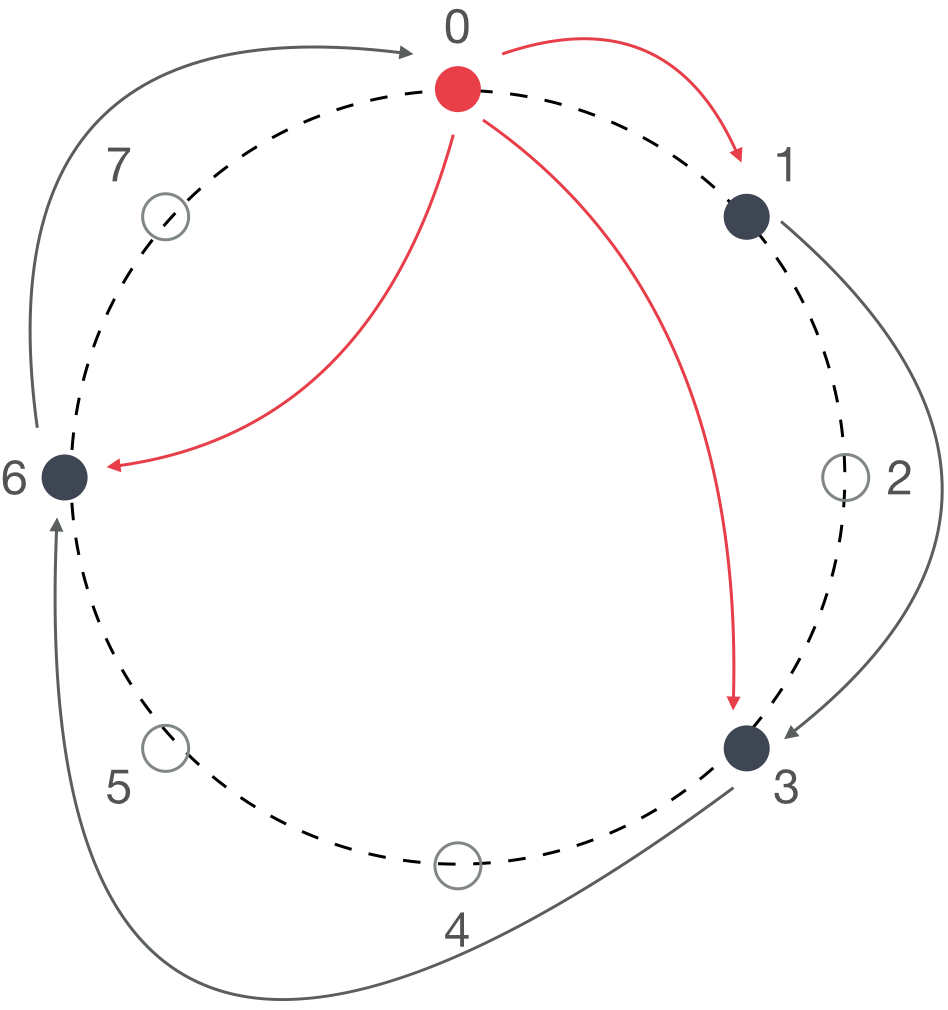
\includegraphics[width=0.4\textwidth]{figs/chord-5}
  \caption{Example of peer with ID = 0 fingers}
  \label{fig:c-5}
\end{figure}

\begin{figure}[h!]
  \centering
  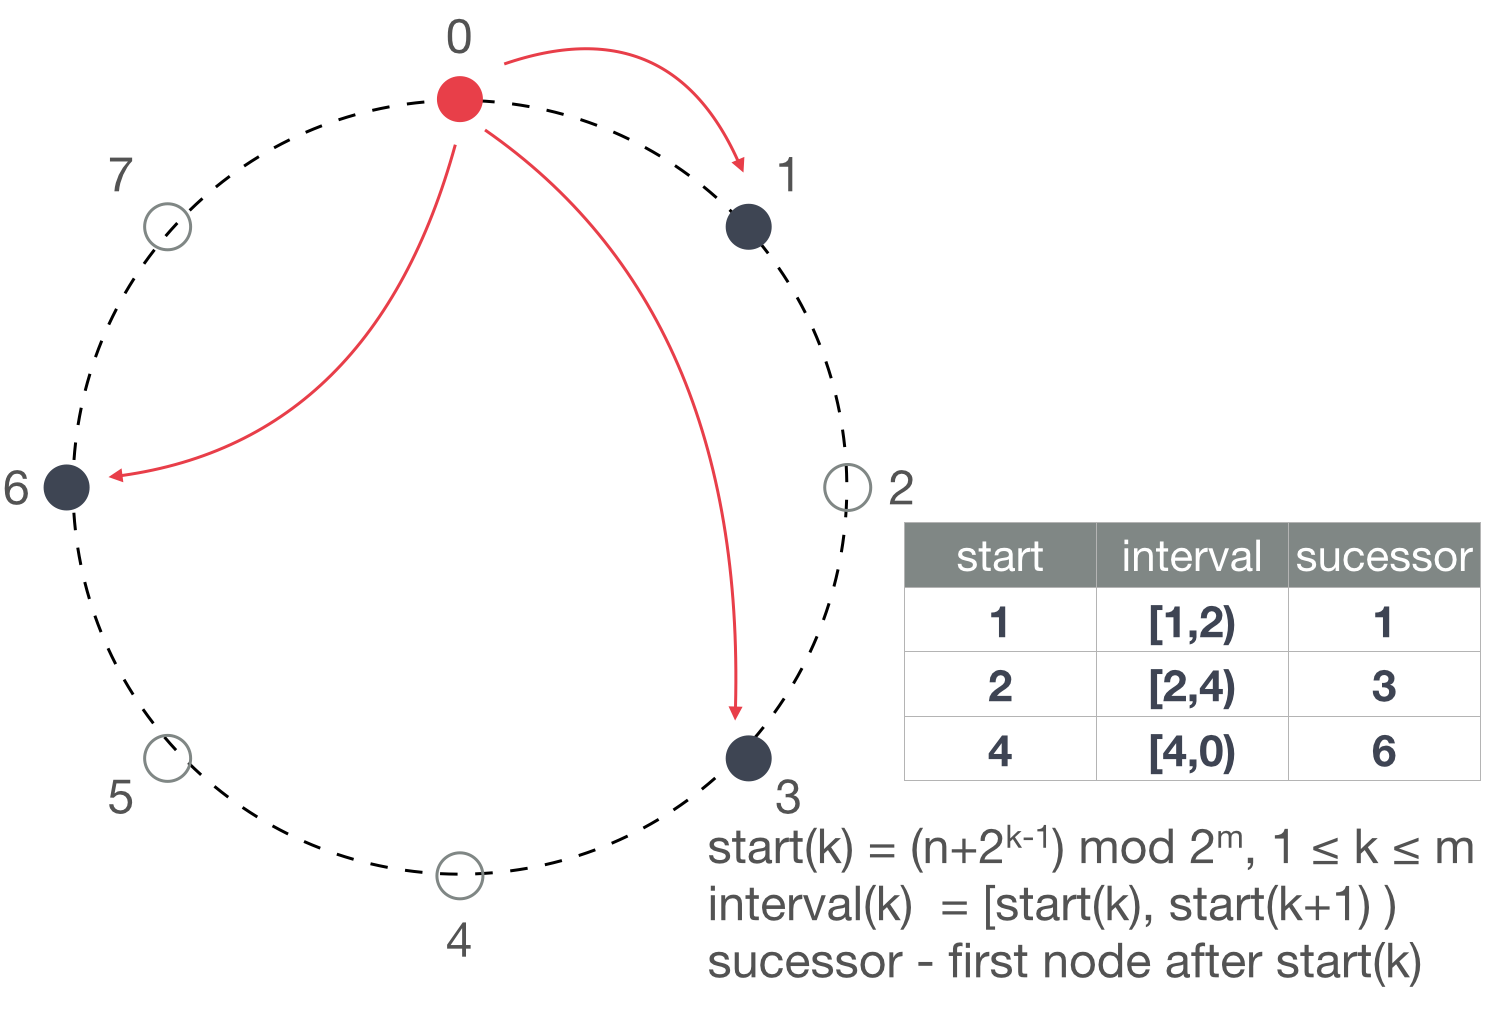
\includegraphics[width=0.4\textwidth]{figs/chord-6}
  \caption{Peer with ID=0 finger table}
  \label{fig:c-6}
\end{figure}

The number of fingers and the fingers we use for a given instance of browserCloud.js are configurable. The reason behind this design decision was that RTCPeerConnections have a significant memory cost, so we have to be considerate in the number of data channels we keep open. In order to give greater flexibility to the developer, we allow the option of picking how many rows of the finger table will be filled by the developer creating a browserCloud.js application. This is also perfect since WebRTC is still a working draft and there might be good developments in resource consumption.

\subsubsection{Filling the finger table for optimal minimum number of hops}

*****************************************************************************
*****************************************************************************
*****************************************************************************
******** EXPLAIN HERE WHAT CAN BE THE BEST STRATEGY FOR FINGER PICKING ******
*****************************************************************************
*****************************************************************************
*****************************************************************************


\section{Resource Management}

Leveraging the browser's dynamic runtime was a feature we pursue from the beginning of the design for browserCloud.js. A job is divided into individual tasks that are a composition of the function to be executed plus the data which should serve as input for that task, creating a transportable gridlet that can be migrated between browsers and executed at its final destination.

\subsection{Job Submission}

A job execution is performed using the algorithm as follows:

\begin{itemize}
    \item 1 - Select in how many units we want to divide a job.
    \item 2 - Select how many browsers we want to distribute the job to.
    \item 3 - Query the network for browser available (e.g. that are not performing other jobs at the moment).
    \item 4 - Compose the several units (gridlets) with with task plus data partition.
    \item 5 - Send this gridlets to the network to be routed to the browser that is going to execute them.
    \item 6 - browser compute the results and send them back to the job issuer.
    \item 7 - the browser that submited the job gathers all the tasks results and constructs the job result.
\end{itemize}

\subsection{Job Execution}

A job consists in the partition of tasks which are enriched with data and sent to other peers to be executed, this tasks, which can be represented as functions (job assets), can be defined in runtime, therefore giving a greater flexibility to the developer that is using this system to run the distributed job they want. We can describe the work performed to schedule a job, by the following algorithm:

\begin{itemize}
    \item 1. A user submits a job
    \item 2. The job is divided in smaller computing units, called tasks, each task compromisses of a segment of the data that is going to be processed and the transformation which is going to be applied, that is, a function.
    \item 3. These task and data are created
    \item 4. The peer will request the network for other peers availability, the user has the capability to specify how many peers should be used to process this job. This option is given since different jobs might benefit of more or less partition, depending on the data set.
    \item 5. The peer who submited the job (the peer that is controlled by the user submitting the job) will receive the individual results for each task as they are ready and transmited. Once all of the results are received, they are aggregated and delivered to the user.
\end{itemize}

\section{Architecture of the Software stack}

When it comes to software, we divided our browser application appliance into three separate and fundamental components, namely: Communication layer, Service router and Job scheduler, leaving also the opportunity for these to be extended. We can observe a overview of this architecture in Figure~\ref{fig:s-a-n-l}.

\begin{figure}[h!]
  \centering
  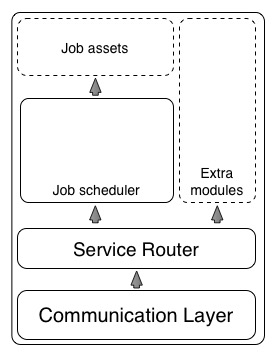
\includegraphics[width=0.4\textwidth]{figs/software-architecture-node-level}
  \caption{Software layers at the peer level}
  \label{fig:s-a-n-l}
\end{figure}


\subsection{Communication layer}

The communication layer is responsible for routing messages between peers and establish a connection with the rendezvous point to perform a peer join/leave. This means that the communication layer:

\begin{itemize}
    \item Holds the connections with other peers.
    \item Performs the necessary logic, using fingers, for efficient routing.
    \item Keeps the peer connected to the network by updating its routing table as necessary
\end{itemize}

\subsection{Service router}

The Service router establishes a protocol for modules like the job scheduler to interact with the network of peers, it uses an event driven model, where modules can register listeners to events that happen on the network (such as a specific reception of a message) and react to it. It also offers the necessary API calls for the modules to send messages to the network.

Service router offers extensibility to browserCloud.js, similar to Job scheduler, other modules can be implemented to interact with the already established P2P network.

\subsection{Job scheduler}

The Job scheduler benefits the API of the Service router to implement its logic, this means that although a job scheduler was implemented to fit our design purposes, it could easily be replaced by another job scheduler with different offers and guarantees.

\section{API design}

For the user of browserCloud.js, a simple API was created to perform: peer join, message listening and job scheduling as demonstrated by the following code (which should be interpreted as pseudo-code since the API might change with the release of new versions):

\subsection{API calls signatures}

\textit{Function signatures}
\begingroup
\scriptsize
\begin{verbatim}
    peer.register(); // Register this peer in the network

    peer.participate(<configuration object>);
    // configuration object should include the URL of the Signalling Server which serves as a rendezvous point for the browserCloudjs instance we want to run our job on. 

    peer.execute(<data for the job>, <task that shall be run for each item on the input data set>, <number of peers we want to distribute our job on>, <callback for when the job is finished>);

\end{verbatim}
\endgroup

\textit{Events signatures}
\begingroup
\scriptsize
\begin{verbatim}
    peer.events.on('registered', <callback>);
    peer.events.on('ready', <callback>);
    peer.events.on('message', <callback>);

\end{verbatim}
\endgroup

\subsection{API Usage Flow}

\textit{Peer join}
\begingroup
\scriptsize
\begin{verbatim}
    // browserCloud.js browser module name is called webrtc-explorer.

    var Explorer = require('webrtc-explorer'); 
    
    var config = {
        signalingURL: '<signalling server URL>'
    };

    var peer = new Explorer(config);

    peer.events.on('registered', function(data) {
        console.log('registered with Id:', data.peerId);
    });

    peer.events.on('ready', function() {
        console.log('ready to send messages');
    });

    peer.register();
\end{verbatim}
\endgroup

\textit{Listen for messages}
\begingroup
\scriptsize
\begin{verbatim}
    // The only action that has to be performed is listen for the message event 
    peer.events.on('message', function(envelope) {
        console.log(envelope);
    });
\end{verbatim}
\endgroup

\textit{Execute a job}
\begingroup
\scriptsize
\begin{verbatim}
    var browserProcess = require('webrtc-explorer-browser-process');

    var config = {
        signalingURL: 'http://localhost:9000'
    };
    
    // Make this browser available to execute tasks and also prepared to issue jobs to the network
    browserProcess.participate(config);

    var start = function() {
        var data = [0,1,2,3,4,5,6,7,8,9,10];  // simple data input
        var task = function(a) {return a+1;}; // e.g of a task (
        var nPeers = 2; // number of peers we are requesting from the network to execute our job
        
        browserProcess.execute(data, task, nPeers, function done(result){
            console.log('Received the final result: ', result); 
        });
    };
\end{verbatim}
\endgroup

\section{Testing framework requirement}

As a collateral but relevant and fruitful effort, we have also designed a testing framework, in order to be able to cope with browserCloudjs needs for quality assurance. 

There are a panoply of excellent browser testing frameworks and services available today, however their focus is on testing browser implementations, namely CSS, HTML and JavaScript, and user interactions of the apps their are testing (e.g. clicks, mouse movements, what the user sees on the page).

When it comes to testing to test a decentralized browser app or library, the focus stops being how a browser implements a specific behaviour, but how the decentralized network handles node joins and leaves and if nodes are effectively communicating between each other. In this scenario, we have several events that the server never sees or that the server never instructs the clients to do, so we need to create a new way to coordinate the browser joins and leaves and also how they interact between each other remotely.

There are a specific set of requirements we needed our testing framework to fulfil, these are:

\begin{itemize}
    \item Have N browsers available, where 1<=N<=virtually unlimited - Most browser testing services only let you spawn a couple of browsers at a time, our solution aims to launch several browsers and/or tabs to load a webpage.
    \item Serve a custom web page for the desired test - So that the developer does not have to provision it before hand and for each test..
    \item Instruct browsers on demand - The ability to send commands to be executed by each browser, depending on the type of test we are running and what events have triggered so far.
    \item Gather information and evaluate the state as a whole - collect the events and data generated by each browser and assess if the order was correct with pseudo external consistency.
\end{itemize}

\subsection{browserCloudjs quality test workflow}

In order to evaluate that a browserCloudjs instance is working as desired, we've designed the following workflow, which can also be seen in Figure~\ref{fig:t-f-1}:

\begin{itemize}
    \item 1 - A Web Server is started by the Control Center, serving the static assets that container our browserCloudjs module that will be run in a browser.
    \item 2 - The number of required browsers for the test being executed, are spawned. In our example in Figure~\ref{fig:t-f-1}, we see that number is 2.  
    \item 3 - Once the browser loads the web page containing the browserCloudjs module, the Control Center starts sending commands to each browser to execute.
    \item 4 - Since the messages and data transfered between browsers happens in a side channel, browsers report to the Control Center which events were triggered.
    \item 5 - Once all the commands were executed, the Control Center assesses the order in which these events happened and asserts if the behavior was the expected.
\end{itemize}

\begin{figure}[h!]
  \centering
  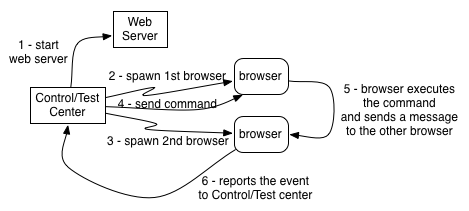
\includegraphics[width=0.7\textwidth]{figs/testing-framework-1}
  \caption{Normal execution of a browserCloudjs test}
  \label{fig:t-f-1}
\end{figure}

\subsection{browserCloudjs quality test assessment} 

browserCloudjs tests are not linear, a message can be routed between any two browsers through several combinations, depending on the current size of the network and the respective IDs of those browsers, which will influence how their finger table looks like.

In Figure~\ref{fig:t-f-2}, we have an example of two browsers communicating between each other. We can see that some of the browser between will have the responsability to forward the message, while others, will be idle. With the design of the testing framework, we wanted to make sure we have a way to take a snapshot of the events that happened in the DHT, so that we can infer if the message was forwared throught the right peers, by analysing each peer finger table.

\begin{figure}[h!]
  \centering
  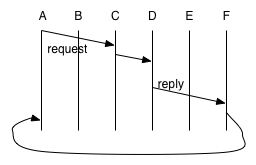
\includegraphics[width=0.7\textwidth]{figs/testing-framework-2}
  \caption{Possible timeline of events for an request from browser A to browser D and the consequent reply}
  \label{fig:t-f-2}
\end{figure}

\section{Summary}

In this section, we covered the network topology of browserCloud.js, which and how interactions are performed and how a developer can use this system.

    %%!TEX root = ../document.tex
\chapter{Implementation}\label{ch:implemenation}

\begin{quotation}
"Tiny modules built on other tiny modules to make tiny powerful high level abstractions".
{\small\it -- James Halliday (substack), founder of browserling, prolific Node.js developer}
\end{quotation}

During the process of developing browserCloud.js, several attempts were created following the Agile methodology, rapidly creating working prototypes and iterating over them. This led to the creation of several open source modules, MIT licensed, having been downloaded in the order of dozens of thousand times until the creation of this document.

Every code artifact was developed following the Unix philosophy, every module attempts to do at most one thing and one thing well, creating small, maintainable and powerful abstractions.

In this section, we describe the implementation details of the final code artifacts that compose the browserCloud.js and the collaterals designed and created that although not projected in the beginning, were needed in order to collect the data we were looking to study.

\section{Browser module}

The browser module is the agent that sits inside our browser nodes, implementing all the communication protocols designed for the browserCloud.js platform and exposing a developer API to send and receive messages.

Essentially it is broken down into 4 components

\begin{itemize}
    \item channel manager - a code artefact responsible to levarage the websockets connection with the signalling server and abstracts the necessary work to open new RTCPeerConnections with other peers.
    \item finger table manager - where the information about a specific peer finger table lives.
    \item router - the routing logic to deliver the messages on the most efficient way. It uses finger table manager to understand what is the most efficient way.
    \item interface - developer exposed interface.
\end{itemize}

The browser module exposes a factory method, meanthing that a developer can instantiate several instances inside a browser.

There are two technologies used in this module, other than the raw Javascript APIs that the browser offers, these are:

\begin{itemize}
    \item browserify - enables the development of browser Javascript code in a modular fashion using the CommonJS standard, such as Node.js does, this means we can require('modules') and create concat and minify our Browser module, so that it can be loaded inside a webpage through a normal <script> tag.
    \item socket.io - socket.io is the most reliable and famous open source implementation of WebSocket API for the browser..
\end{itemize}

\section{Signalling server}

The signalling server offers two Web APIs, one being a WebSockets API and the other a RESTful API. The design decision behind these two APIs was mainly because since the network evolves with time, we needed a way to be able to push, on demand, new information to browsers, for example, when a new peer needs to be railed in, or when the Signalling Server acts as a rendezvous point for SDP data exchange between browsers so they can establish a RTCPeerConnection.

The second API, RESTful, is used to instruct the server or to collect analytics data from it remotely.

\section{Key learnings from the earlier iterations - webrtc-ring}

During one of the earlier iterations, we've developed a prototype of webrtc-explorer, called webrtc-ring, which although very similiar in routing strategy, each peer only knew about its successor, in another words, each peer only had access to one finger, this originated a system with the following properties:

\begin{itemize}
    \item overlay structure - 1 dimension Hash Ring
    \item lookup protocol - Matching key and NodeID
    \item network parameters - Number of Nodes in the network
    \item routing table size - 1
    \item routing complexity - O(log(N))
    \item join/leave overhead - 2
\end{itemize}

During the development, we performed tests to evaluate the capacity of the system to distribute work, later discussed on the Evaluation section. We learned that due to the single thread nature of Javascript, running message routing inside the same process that would be use to perform CPU bound tasks could be highly disavantageous for browserCloud.js performance. To overcome this, we introduced Web Workers to the system, independent threads inside the browser to separate communication from CPU bound tasks.

\section{Implementation collaterals}

During the development of the browserCloud.js system, several tools were built in order to properly test components of the system, or to perform performance analytics. These needed to be designed from the ground up due to browserCloud.js peculiar nature.

\subsection{Testing browserCloud.js}

There are a panoply of excellent browser testing frameworks and services available today, however their focus is on testing browser implementations (CSS, HTML and JavaScript) and user interactions of the apps their are testing (clicks, mouse movements, what the user sees).

When it comes to testing to test a decentralized browser app or library, the focus stops being how a browser implements a specific behaviour, but how the decentralized network handles node joins and leaves and if nodes are effectively communicating between each other. In this scenario, we have several events that the server never sees or that the server never instructs the clients to do, so we need to create a new way to coordinate the browser joins and leaves and also how they interact between each other remotely and this is were piri-piri comes into play.

The specific set of problems piri-piri tries to solve:

\begin{itemize}
    \item browser times X, where 1<=X<=virtually unlimited - Most browser testing frameworks only let you launch a couple of browsers at a time, piri-piri aims to launch several browsers and/or tabs to load a webpage, in a local or distributed fashion.

    \item instruct browsers on demand - Since there is a ton of stuff happening on browser decentralized apps, we can't just write a script to test and listen to events that happens in a single browser, there are triggers coming from all of them.

    \item gather information and evaluate the state as a whole - collect the events and data generated by each browser and assess if the order was correct with pseudo external consistency
\end{itemize}

\subsection{Visualize the network state}

Using D3JS, a API library that works as a thin veneer on top of SVG, we've developed an application that grabs the state of the browserCloud.js network and shows a live graphical representation, as seen on Figure~\ref{fig:visualizer}, where each node is represented by a dot and its ID and the arcs being the connections established between the nodes in the network.

\begin{figure}[h!]
  \centering
  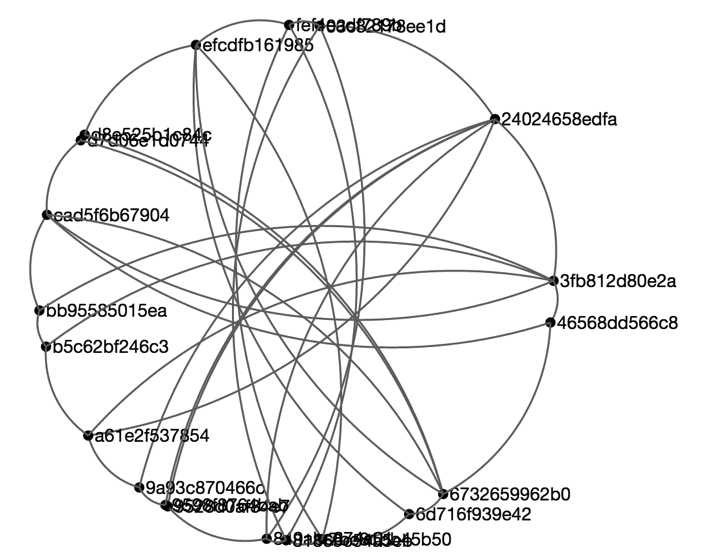
\includegraphics[width=0.7\textwidth]{figs/visualizer}
  \caption{Visualization of a browserCloud.js network}
  \label{fig:visualizer}
\end{figure}

\subsection{Simulate a browserCloud.js network}

In addition to the visualizer application, one simulator application was developed, were not only a graphical representation is generated, but also, it gives the developer a way to create a new virtual network, without any real peers. We've the option to pick the number of peers we want present and how many and which fingers will be used, so we can analyse different distribution paths and optimize for number of hops between any two peers in the network.

\subsection{Ray Tracing module}

To perform the parallel CPU bound tests, we've developed a module that works in Node.js and in the browser to perform Ray Tracing Tasks. The module works in a synchronous fashion so it performs faster, in another words, there are not techniques to make que module asynchronous that would create an overhead for the processing, in order to avoid stopping javascript event loop, the ray tracing task has to be ran in a sub process.

This module performs the interpretation of a scene designed in CSS, division of the scene in multiple parts (tasks) and reconstruction of the ray traced scene when every task is completed.

\section{Summary}



    %%!TEX root = ../document.tex
\chapter{Evaluation}\label{ch:evaluation}

\begin{quotation}
  {\small\it }"ANOTHER FANTASTIC QUOTE"{\small\it -- FROM SOMEONE FANTASTIC }
\end{quotation}


In this section we evaluate browserCloud.js via real executions on top of increasing number of browsers executing locally, to assess the limits of current Javascript engines on typical desktop machines, and with micro-benchmarks to determine the speedups that can be achieved in distributed executions with one browser per individual desktop machine.

This, in order to assess the potential of the proposed system, we have built a ray-tracing application, adapted from algorithms available, written in full vanilla JavaScript, that can be run on any  typical modern browser engine. This algorithm allows us to stress-test the CPU,  and the possibility to obtain advantages through processing parallelism. We need this to understand whether the expected speeds up resulting from distributing the tasks through the browserCloud.js peers network, are not hindered by loosing efficiency due to message routing on the overlay Network.

When distributing a job through a multiple node network, one of the aspects we observed was that we can influence overall efficiency by adjusting how much resources we are going to take from the network to process the job, in this case, how much browsers. We also can influence it by deciding how much fine-grained each task it will be: the smaller the computation unit, the more we can distribute tasks through the network, with a natural trade-off of adding more task generation and messaging overhead, with diminishing returns when more and more, and  smaller tasks are created.

The standard ray-tracing job using the algorithm developed, running in a single browser takes as median 2361.434s to complete (around 40 minutes). As we can see in Figures~\ref{fig:ray2500}~and~\ref{fig:ray2500time}, our system excels in delivering faster results by dividing the job up to 2500 computational units (or tasks) and requesting from the browsers available in the network to compute those (i.e., a rectangle of the resulting output image). This is expected as ray-tracing is a known case of an embarrassingly parallel application.

One fact interesting to note is that we obtained much better results by reducing the granularity of which ray-tracing job was divided into, as we can see on Figures~\ref{fig:ray25}~and~\ref{fig:ray25time}. This happens due to two factors: a) the first is that since we have a lower number of tasks to be run by other browsers, we reduce the message routing overhead between nodes (i.e., resource discovery does not take so long); b) the second factor is that since this system was tested using a single machine and a networked simulated delay. When the number of tasks is too large, the workers in the browser are in fact competing for CPU resources (to execute tasks and to forward messages among them). This creates a scenario, where more nodes/workers actually  make the system slower, since this is a much more strict and resource constrained scenario, than a real example with browsers executing in different machines.

In a real world example, the actual execution time would be bounded by:\\

$\textbf{jobTime}=slowestDelayFromResourceDiscovery+timeOfExecutingSlowestTask+slowestDelayFromResultReply (1)$ \\

with full parallelism, where in our test scenario we have: \\

$\textbf{jobTime}=\sum{DelayFromResourceDiscovery}+(TimeOfExecuting\_N\_Tasks\_on\_M\_Resources)+\sum{DelayFromResultReply} (2)$\\

where N=2500 and M=8 hardware threads, therefore contention for CPU becomes higher with more nodes (browsers) as more messaging is taking place, besides the parallelized computation.

\begin{figure}[]
  \centering
  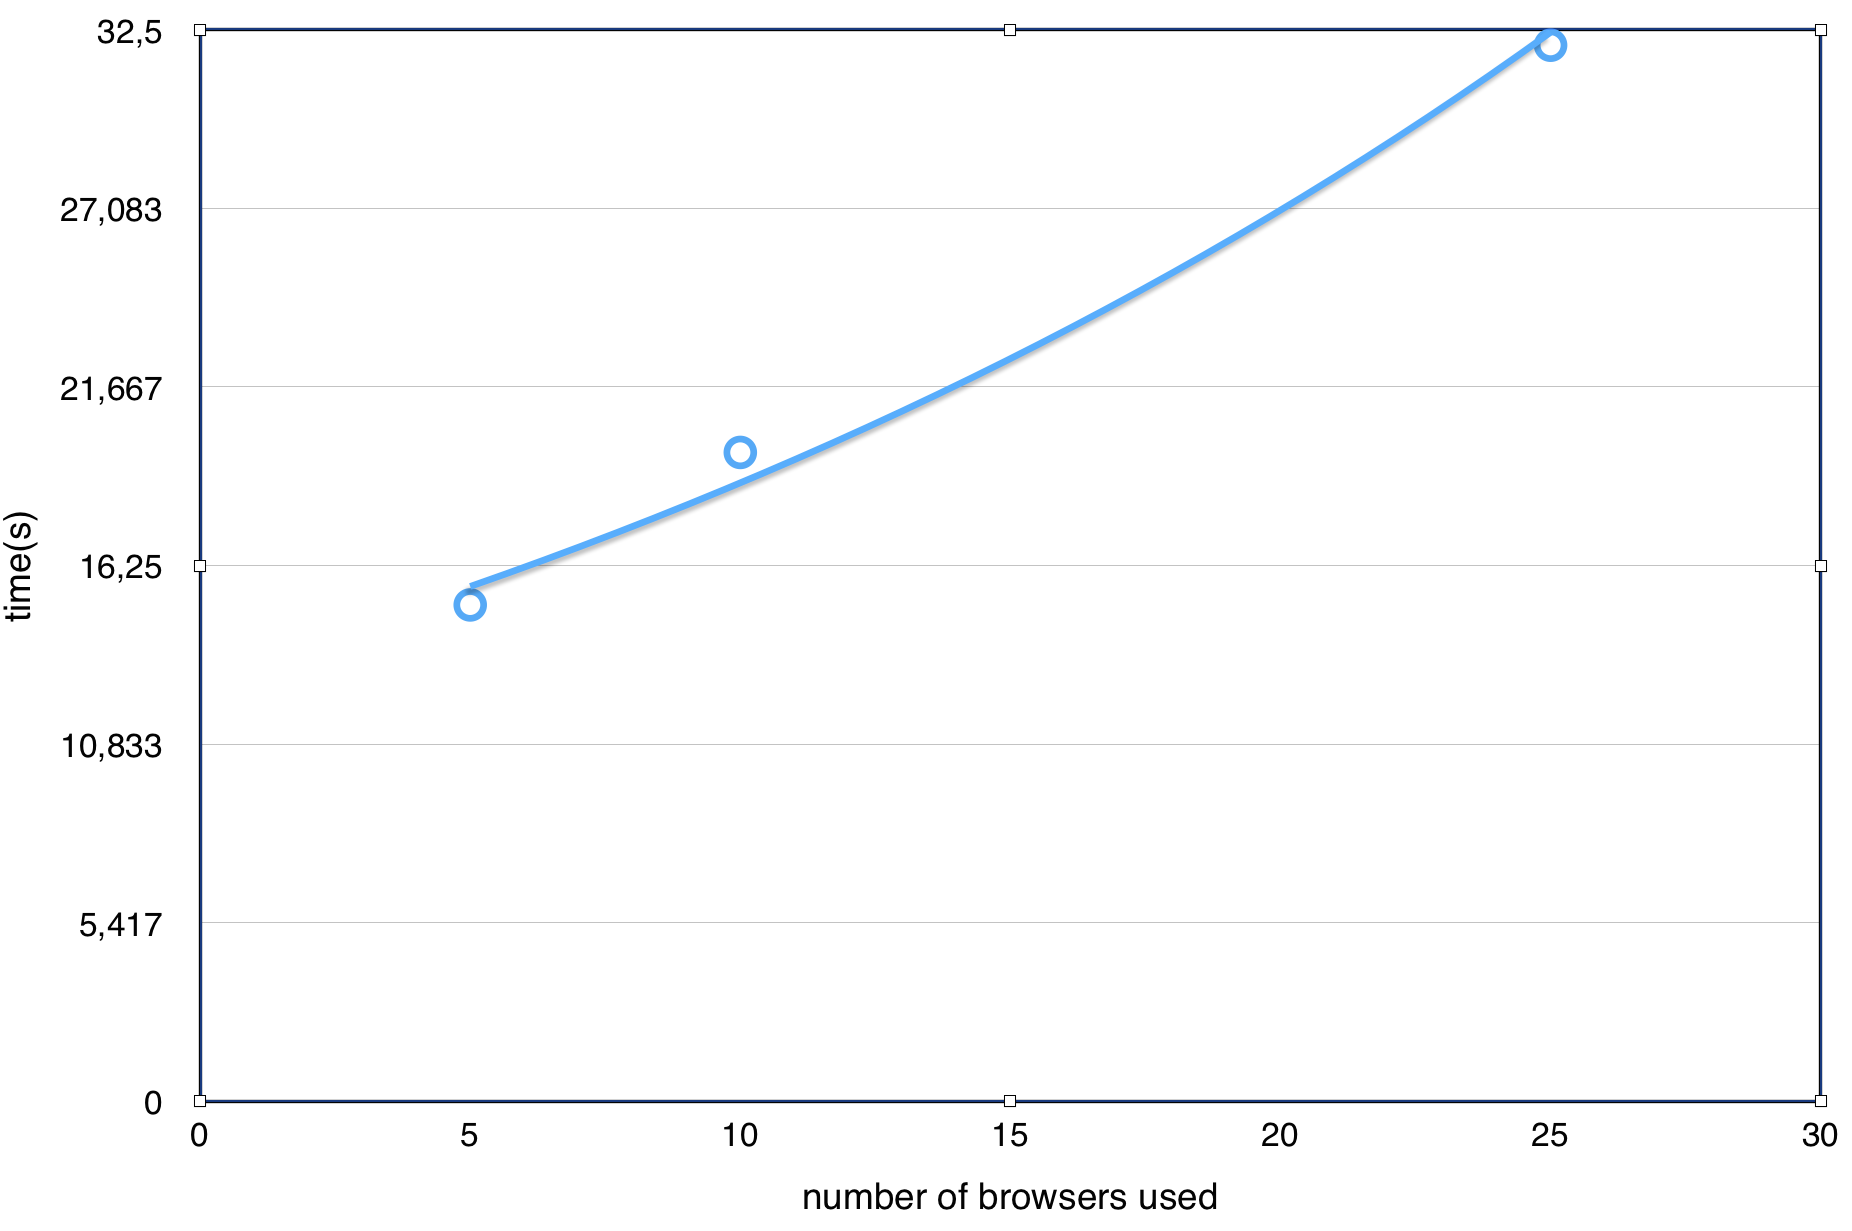
\includegraphics[width=0.8\textwidth]{figs/1.png}
  \caption{Time elapsed on a ray-tracing job divided in 2500 computing units}
  \label{fig:ray2500}
\end{figure}

\begin{figure}[]
  \centering
  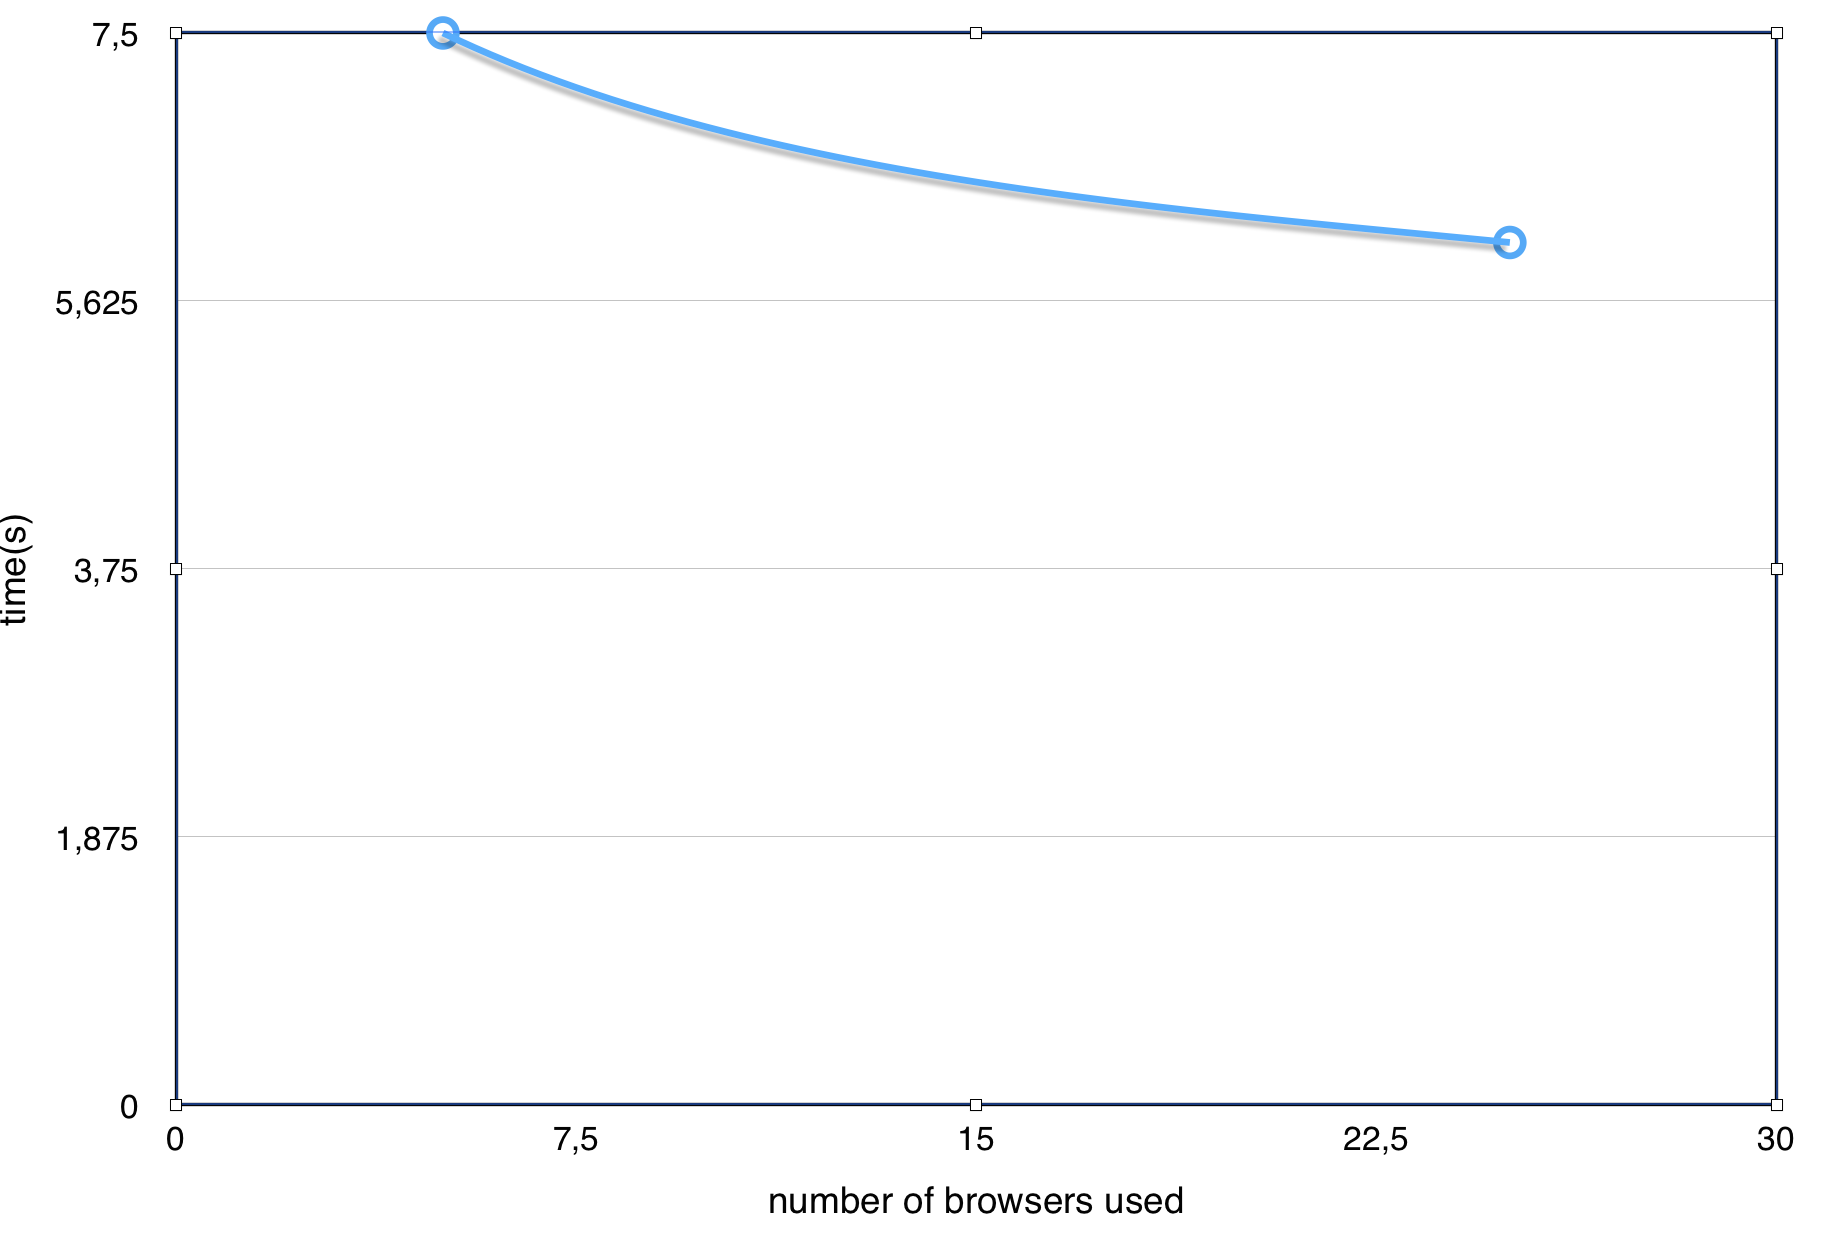
\includegraphics[width=0.8\textwidth]{figs/2.png}
  \caption{Time elapsed on a ray-tracing job divided in 25 computing units}
  \label{fig:ray25}
\end{figure}

\begin{figure}[]
  \centering
  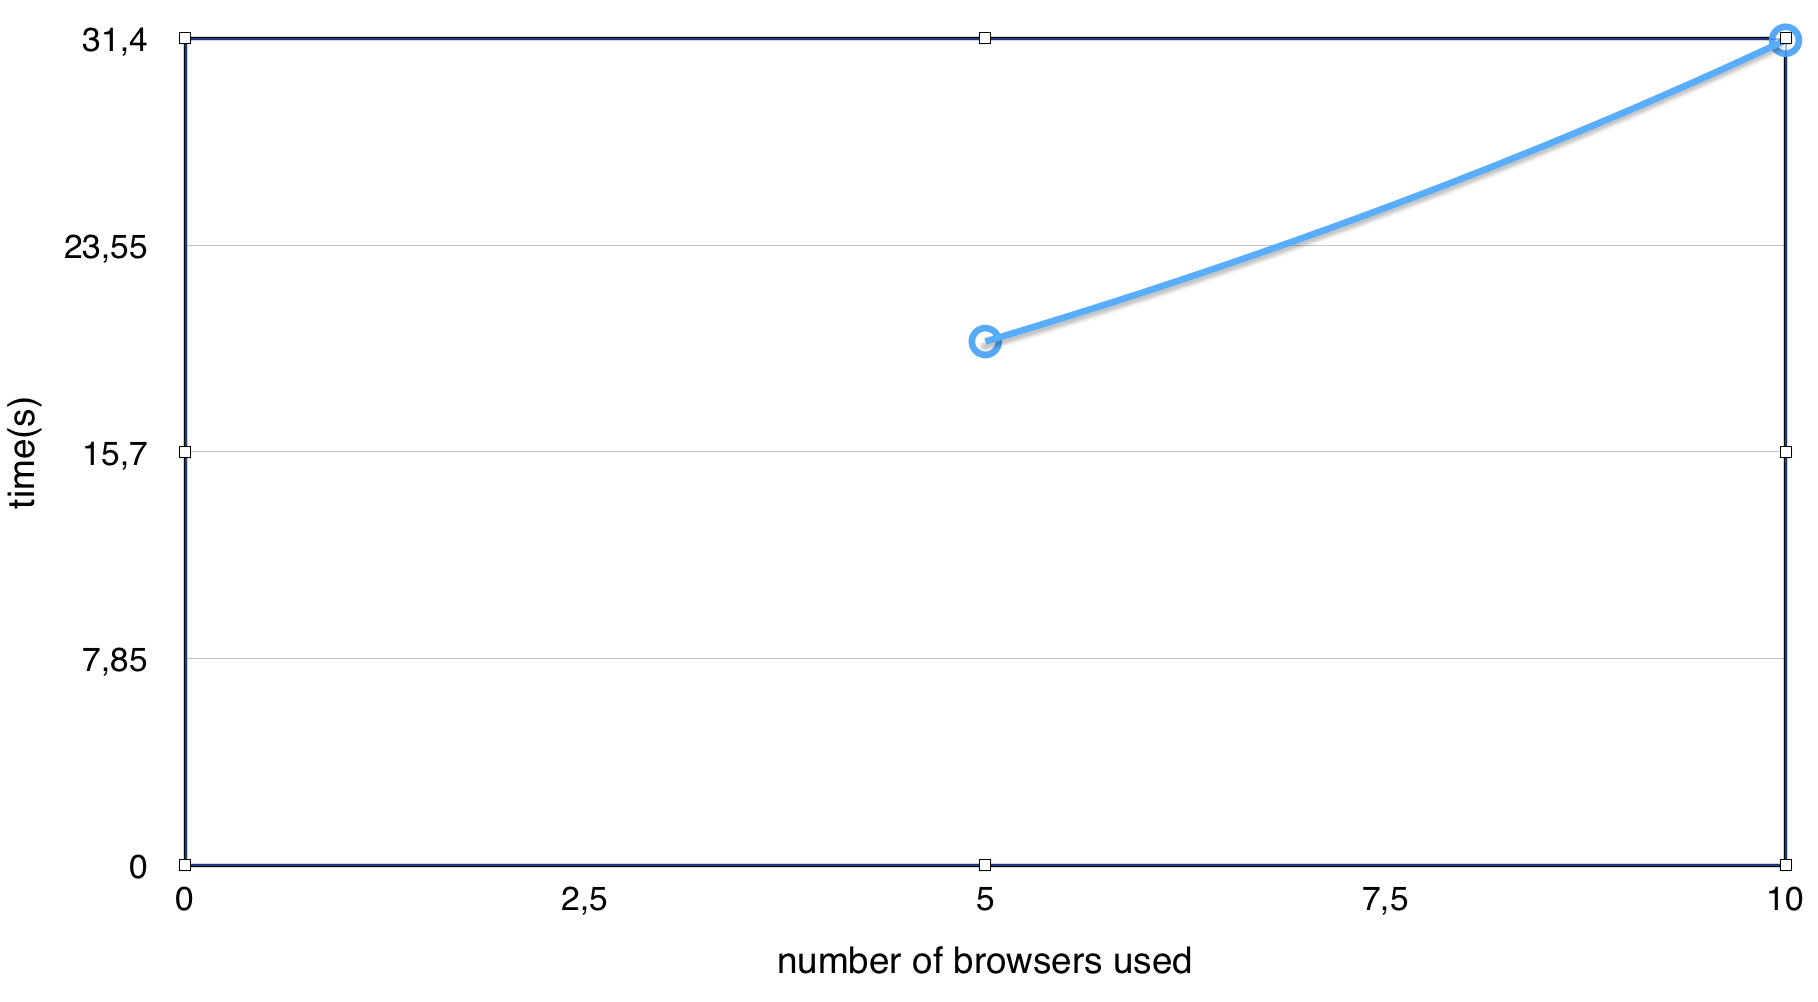
\includegraphics[width=0.8\textwidth]{figs/3.png}
  \caption{Time elapsed on a ray-tracing job divided in 2500 computing units (with induced web RTT delay)}
  \label{fig:ray2500time}
\end{figure}

\begin{figure}[]
  \centering
  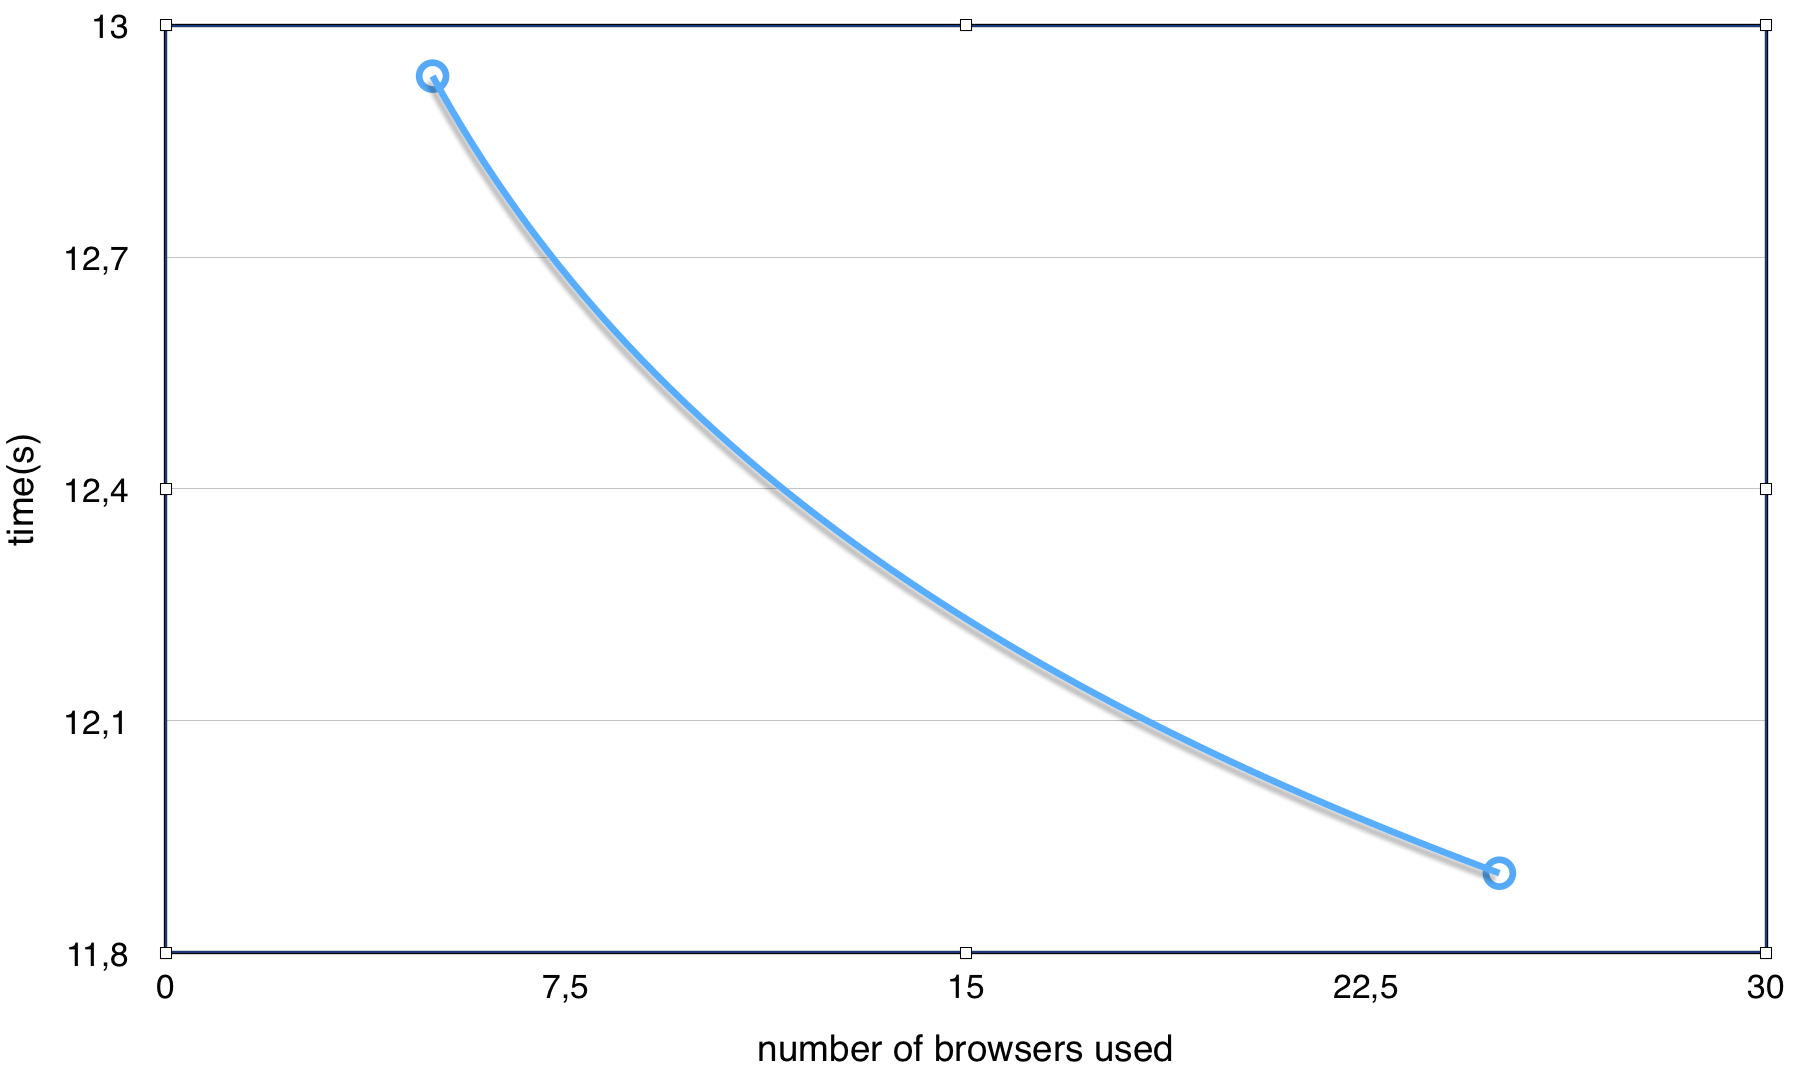
\includegraphics[width=0.8\textwidth]{figs/4.png}
  \caption{Time elapsed on a ray-tracing job divided in 25 computing units (with induced web RTT delay)}
  \label{fig:ray25time}
\end{figure}

In a real world scenario, with more browsers from more machines, the total execution time (makespan) of a ray-tracing job would be closer to that described by Equation 1. It would be influenced by the maximum round trip time between any two nodes (so that the information for every task can be received and processed by another node), plus the time it would take to execute the most of CPU intensive task (e.g., the rectangle in the frame that has the more complex geometry and light reflections to be processed). Figures~\ref{fig:avgtimeexec}~and~\ref{fig:rtt} show what is the average task length and RTT between any two nodes, being the maximum for the first 61ms and the second 11174ms, creating a total of 11235ms (or 11.296s overall). This is a significant increase of efficiency, comparing to the sequential execution (a speedup of about 209 times fold) and also to the previous single-machine experiments.

It is important to note that in Figure~\ref{fig:avgtimeexec}, we can see several task execution lengths due to the complexity of each task, with more or less light reflections. With this microbenchmark we see that the execution time of each task, without any resource contention (1 node = 1 browser per machine), the task duration has an even lower upper bound (lower than 5s). This would entail the upper bound of total task execution time to be under 5061 ms (around just 5s), with a theoretical speedup of about 466 times (take into account that we would be using 2500 nodes then, so speedups are not perfectly linear due to communication overhead, as expected).

\begin{figure}[]
  \centering
  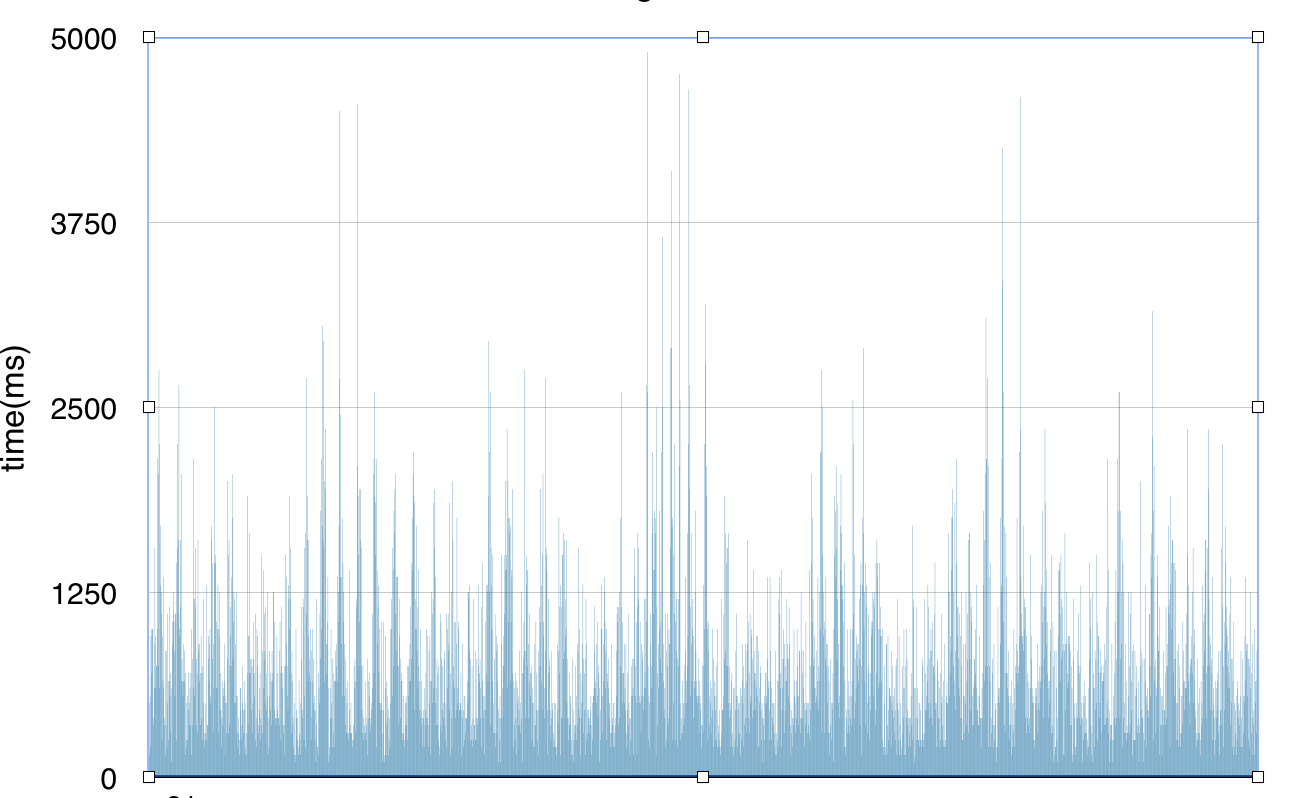
\includegraphics[width=0.8\textwidth]{figs/avg_time_exec.png}
  \caption{Average time for a task execution for a job fragmented in 2500 computing units}
  \label{fig:avgtimeexec}
\end{figure}

\begin{figure}[]
  \centering
  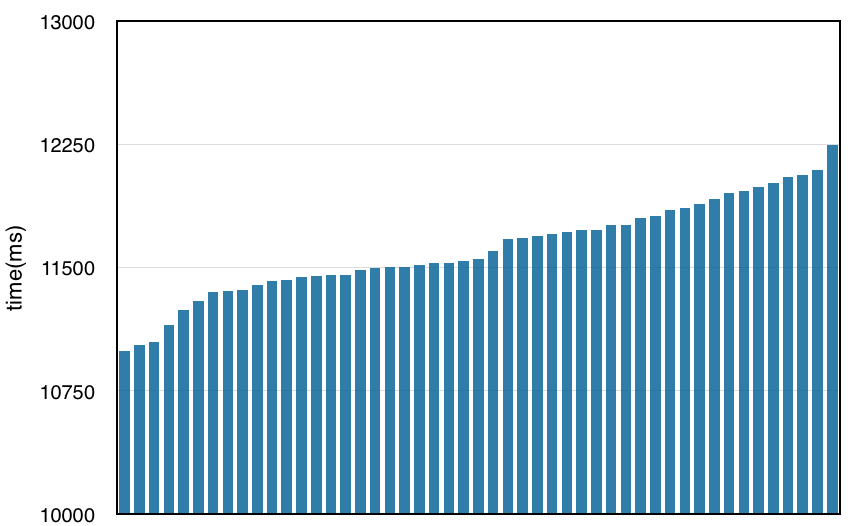
\includegraphics[width=0.8\textwidth]{figs/rtt.png}
  \caption{Average Round Trip Time between an two nodes in a 10 browser network}
  \label{fig:rtt}
\end{figure}


There are also some other performance bottlenecks we noticed that arise from the single threaded nature of JavaScript engines. These aspects are considered in our performance evaluation, such as:

\begin{itemize}
  \item Logging - Since V8 runs in a single thread, any synchronous operation will block the event loop and add delay to the whole processing, although these logs are essential for us to assess the efficiency of the infrastructure, they are not vital to the job.
  \item Delay added - One technique we used to simulate the network delay is to use the `setTimeout' native function of V8's JavaScript implementation, since this function is unable to receive floating millisecond values. Moreover, since `setTimeout' does not necessarily guarantee that the function will be executed in X amount of milliseconds, due to the nature of the event loop, there is always an extra delay added implicitly to the operation in the order of 1 to 3 ms.
  \item Tasks can not be sent in parallel - A node has to send each individual computing unit sequentially and independently, meaning that if we divide a job into 2000 for e.g, each task will have to wait for the previous to be sent.
\end{itemize}

These bottlenecks were studied and will be tackled in future work, one of the solutions proposed is to use Service Workers\cite{ServiceWorkers} for full multithreaded operation inside browserCloud.js.


\section*{Summary}

    %%!TEX root = ../document.tex
\chapter{Conclusion}\label{ch:conclusion}

\begin{quotation}
  "In the end, it's not the years in your life that count. It's the life in your years."
  {\small\it -- Abraham Lincoln}
\end{quotation}

We end this report, making an overview and summing up all the primary aspects, from proposed work, contributions, state of the art, definition of the architecture, implementation of the respective architecture and evaluation, moving to what were the major breakthroughs and ending with concluding remarks and future work.

People sharing resources is one of the oldest sociological behaviors in human history, however although some known attempts as SETI@HOME (even if extended with nuBOINC) have enabled that for our computer machinery, the level of friction that has to be made in order for a user to join, has been significantly high to cause a great user adoption. On the other hand, Open Cloud stacks have been evolving, providing nowadays the most reliable and distributed systems performance, having a bigger adoption even if the resources are geographically more distant or expensive.

browserCloudjs was an exercise to strive towards a federated community cloud, enabling its users to share effectively their resources, giving developers a reliable and efficient way to store and process data for their applications.

When it came to architecture decisions, we knew that we wanted to built browserCloudjs on top of the most recent web technologies and on top of the Web Platform, the most ubiquitous platform. There were two reasons behind this decision, the first being longevity, the Web Platform, even though it is quite popular, it is still an emerging platform, meaning that our assumptions of ubiquity will previal; the second reason was developer adoption, JavaScript is the "lingua franca" of the web, meaning that it will be common for a developer to know how to code with JavaScripts APIs and since browserCloudjs was built in JavaScript, developers will know inherently how to use the platform.

Going after a decentralized model was also something we saw as a potential key factor for the browserCloudjs platform, structured peer-2-peer networks scale well with demand, while centralized networks have a number of significant challenges once a certain threshold of users is reached. WebRTC, the technology enabling browsers to communicate in a peer-2-peer way, is in great part responsible for this platform success.

With browserCloudjs, we achieved in bulk, mainly two great milestones:

\begin{itemize}
    \item \textbf{The first browser based DHT} - browserCloudjs offers for the first time in browser history a fully functional DHT, performing resource decentralized resource discovery on the browser. 
    \item \textbf{The first peer-2-peer browser computing platform} - the research of using browsers to leverage the idle computer cycles have been in the literature for a while, however, always following the centralized/BOINC model. browserCloudjs offers the first peer-2-peer browser computing framework with proven speedups.
\end{itemize}

We have found this thesis to be a source of hard work and enthusiasm, a great opportunity to research and interact with bleeding edge technologies and also, interact with the developer communities that are pushing the web forward. From this work results a collection of items that we see as future work, described in the following section.

\subsection{Future Work}

As future work for our research, we've identified some areas that we believe that would contribute to the goal of the platform, these are:

\begin{itemize}
    \item New job strategies - Currently browserCloudjs only supports mapping jobs, however, there is no pratical limitation to execute full map/reduce jobs and/or streaming functions (for realtime data scenarios).
    \item Hybrid peers - peers that live inside of a server that can both act as a signalling server and stabilizing the network when the churn rate is high.
    \item Geographic distribuiton awareness - Select finger tables based in optimal RTT distribution and geographic positioning of peers.
    \item Optimization of the JavaScript code developed - Increasing the performance of crucial functions.
    \item Continuous upgrade of browserCloudjs platform as the Web Platform APIs evolve and as WebRTC moves from the draft state to finished spec.
\end{itemize}

    %\input{sections/11_future}
    %
    \newpage
    \thispagestyle{empty}
    %!TEX root = ../document.tex

\bibliographystyle{chicago}
%\bibliographystyle{plain}
%\bibliographystyle{ieeetr}

\bibliography{bibliography}


    \appendix

    \begin{singlespace}
        \def\indexname{Index}
        \printindex\cleardoublepage
    \end{singlespace}
\end{document}

